\documentclass[11pt,a4paper]{article}

% Page layout
\usepackage[a4paper,margin=2.7cm]{geometry}

% Engine-aware Unicode + Russian
\usepackage{iftex}
\ifPDFTeX
  \usepackage[T2A]{fontenc}
  \usepackage[utf8]{inputenc}
  \usepackage[russian,english]{babel}
\else
  \usepackage{fontspec}
  \usepackage{polyglossia}
  \setdefaultlanguage{russian}
  \setotherlanguage{english}
  \defaultfontfeatures{Ligatures=TeX}
  \setmainfont{Latin Modern Roman}
  \setsansfont{Latin Modern Sans}
  \setmonofont{Latin Modern Mono}
\fi

% Typography + math
\usepackage{microtype}
\usepackage{mathtools}
\usepackage{amssymb,amsfonts}
\usepackage{amsthm}
\usepackage{bm}

% Emergency stretch
\setlength{\emergencystretch}{2em}
\usepackage{float}

% Common operators / constants
\DeclareMathOperator{\Tr}{Tr}
\newcommand{\ii}{\mathrm{i}}
\newcommand{\dd}{\mathrm{d}}

% Figures/tables
\usepackage{graphicx}
\usepackage{booktabs}
\usepackage{longtable}

% Lists
\usepackage{enumitem}

% Quotes (needed for biblatex in many setups)
\usepackage{csquotes}

% Theorem-like environments
\theoremstyle{definition}
\newtheorem{definition}{Определение}[section]
\newtheorem{axiom}{Постулат}[section]
\theoremstyle{plain}
\newtheorem{proposition}{Утверждение}[section]
\newtheorem{lemma}{Лемма}[section]
\theoremstyle{remark}
\newtheorem{remark}{Замечание}[section]

% Bibliography (biblatex + biber)
\usepackage[
  backend=biber,
  style=numeric-comp,
  sorting=none,
  maxbibnames=99
]{biblatex}
\addbibresource{references.bib}

% Hyperlinks: load hyperref late; cleveref after hyperref
\usepackage[unicode,hidelinks]{hyperref}
\usepackage{bookmark} % improves PDF bookmarks stability
\usepackage[nameinlink,noabbrev]{cleveref}

% cleveref names for theorem-like environments
\crefname{axiom}{постулат}{постулаты}
\Crefname{axiom}{Постулат}{Постулаты}

\crefname{definition}{определение}{определения}
\Crefname{definition}{Определение}{Определения}

\crefname{proposition}{утверждение}{утверждения}
\Crefname{proposition}{Утверждение}{Утверждения}

\crefname{lemma}{лемма}{леммы}
\Crefname{lemma}{Лемма}{Леммы}

\crefname{remark}{замечание}{замечания}
\Crefname{remark}{Замечание}{Замечания}

% Better Russian names in cleveref
\crefname{equation}{уравнение}{уравнения}
\Crefname{equation}{Уравнение}{Уравнения}
\crefname{figure}{рис.}{рис.}
\Crefname{figure}{Рис.}{Рис.}
\crefname{table}{табл.}{табл.}
\Crefname{table}{Табл.}{Табл.}
\crefname{section}{раздел}{разделы}
\Crefname{section}{Раздел}{Разделы}
\crefname{subsection}{подраздел}{подразделы}
\Crefname{subsection}{Подраздел}{Подразделы}

% Title info
\title{Геометрия масштаба сложных систем: формализм и эмпирическая проверка локального \texorpdfstring{$\Lambda_b$--$\Pi_b$}{Lambda_b-Pi_b} замыкания в атмосферных данных}
\author{Sotiriadi N.}
\date{2026}

\begin{document}
\maketitle

\begin{abstract}
Работа проверяет гипотезу о том, что масштаб в сложных системах можно рассматривать как полноценную координату описания, а межмасштабный перенос --- как геометрически организованную динамику, а не как простое усреднение. Для этого вводится калибровочно-инвариантный функционал \(\Lambda_{\mathrm{matter}}\), вычисляемый из кривизны связности и состояния, и рассматривается его локальная полосовая версия \(\Lambda_b\) в операциональном \(\Lambda_b\sim\Pi_b\)-замыкании, где \(\Pi_b\) --- спектральный поток энергии в полосе \(b\).

Проверка выполнена в двух классах данных. На модельном этапе (T20) в инерционном диапазоне получена устойчивая квазилинейная связь \(\Lambda_b\sim\Pi_b\) с \(R^2_{\mathrm{binned}}=0.727\); на краях каскада (подпитка/диссипация) связь ослабевает или меняет знак. На атмосферном этапе (A15, ERA5, окно 2017-01-01~00:00:00 --- 2017-03-31~18:00:00, шаг 6 часов) получен согласованный результат: \(R^2_{\mathrm{binned}}=0.520\), положительный наклон и \(p=0.008\) в инерционном подинтервале при предсказуемом распаде связи вне него.

Дополнительные серии уточняют физическую картину и границы применимости: в процессно-разрешённой ветке A05 на нижнем масштабе требуется память (переход от минимальной модели к GKSL/CPTP-замыканию), а в A11--A14 показано, что перенос на одной плитке неустойчив без физически соседнего окружения.

Итоговый вывод для междисциплинарного чтения таков: предложенный формализм не только внутренне согласован, но и даёт эмпирическую поддержку локального \(\Lambda_b\sim\Pi_b\)-замыкания в реальных атмосферных данных. При этом работа не утверждает универсальное ``подтверждение ОТО в атмосфере'': фундаментальный статус \(\Lambda_{\mathrm{matter}}\) и универсальность замыкания вне режима локальной ячейки остаются открытыми вопросами.
\end{abstract}
\newpage

\tableofcontents

\newpage
\section{Введение}
\label{sec:intro}

\subsection{Мотивация: масштаб, динамика и геометрия}

Практическая отправная точка этой работы --- плохо замыкающиеся балансы в мультимасштабных системах. В задачах атмосферы и климата это проявляется как остатки во влагобюджете и энергетических балансах даже после улучшения разрешения, ассимиляции и параметризаций. Для тестового кейса мы используем задачу WPWP/ERA5, где остаточное замыкание можно измерять напрямую и проверять в блочно-кросс-валидационной постановке \cite{Hersbach2020ERA5,CopernicusC3S2017ERA5,PeixotoOort1992PhysicsClimate,TrenberthEtAl2007WaterBudget}.

Рабочая гипотеза состоит в том, что часть этих невязок связана не только с шумом и несовершенством моделей, но и с некоммутативностью межмасштабных переходов: результат зависит от порядка огрубления и динамического обновления. В такой постановке масштаб перестаёт быть чисто внешним индексом и приобретает операциональный статус дополнительной координаты описания в эффективной модели. Мы используем для этого геометрический язык гильбертова расслоения, где межмасштабный перенос задаётся связностью, а его кривизна порождает диагностические инварианты.

Важно сразу зафиксировать уровень притязаний. Мы \emph{не утверждаем}, что тем самым построена завершённая фундаментальная теория огрубления или новая УФ-динамика. Мы предлагаем исследовательскую рамку, в которой можно последовательно проверять, несёт ли геометрия масштаба воспроизводимую информацию сначала в модельных классах, затем в атмосферных данных.

Отдельно отметим, что такая постановка не возникает в пустом месте и опирается на сильную географическую традицию анализа иерархий. В работах Ю.\,Г.~Пузаченко пространственно-временная организация геосистем рассматривалась как многомасштабный процесс с собственными инвариантами и измеримыми режимами динамики; там же сформулированы ключевые методологические основания для практического анализа иерархических структур в географии и экологии \cite{Puzachenko1986Hierarchy,Puzachenko2004Methods,Puzachenko2010Invariants}. Этот контекст важен для корректного чтения нашего формализма как преемственного расширения, а не изолированной физико-математической конструкции.

Для удобства междисциплинарного чтения, предлагается ознакомиться с \hyperref[sec:appendix:glossary]{Приложением С}, где даны объяснения основных используемых аббревиатур и понятий.

\subsection{Масштаб как координата: гильбертово расслоение}

Основная конструкция работы состоит в том, чтобы рассматривать не одно фиксированное гильбертово пространство, а семейство пространств
$\{\mathcal H_{x,\mu}\}$, параметризованное пространственно-временной точкой $x$ и масштабом $\mu$.
Состояние тогда задаётся \emph{сечением} над расширенной базой, а переходы между масштабами реализуются вложениями и связностью по координате $\mu$.

Такой язык естественно отделяет два вопроса: динамику внутри данного масштаба и перенос между масштабами.
Последний в общем случае не обязан быть коммутативным, и именно эта некоммутативность мотивирует введение калибровочно-инвариантных диагностических объектов вроде $\Lambda_{\mathrm{matter}}$.
Мы используем геометризацию РГ-пространства как рабочую математическую модель, совместимую с идеями $c$-теоремы Замолодчикова и голографического РГ \cite{Zamolodchikov1986Irreversibility,deBoerVerlindeVerlinde2000HolographicRG,RandallSundrum1999LargeHierarchy,RandallSundrum1999Alternative}, но не отождествляем наш модельный объект с уже установленной метрикой пространства теорий.

\subsection{Динамика и вертикальная связность}

На фиксированном масштабе мы используем стандартный язык унитарной или GKSL/Линдбладовской открытой динамики \cite{GoriniKossakowskiSudarshan1976GKSL,Lindblad1976Generators,Kraus1983StatesEffectsOperations,Stinespring1955PositiveFunctions,NielsenChuang2000QCQI,BreuerPetruccione2002OpenQuantum}. Межмасштабный перенос кодируется отдельной вертикальной связностью $A_\mu$, так что эволюция сечения зависит и от времени, и от движения по координате масштаба.

Ключевой момент работы состоит в том, что марковский предел трактуется как базовое приближение, а не как окончательное описание. Физически декогеренция и перераспределение информации между слоями не обязаны быть мгновенными. Именно поэтому в дальнейшем мы отдельно обсуждаем задержку и память на малых масштабах: соответствующая необходимость не вводится аксиоматически заранее, а возникает как эмпирически мотивированное расширение после процессно-разрешённого блока A05.

\subsection{Термодинамические предпосылки и связь с гравитацией}

Термодинамический блок в работе играет роль локального замыкания в контролируемом квазистатическом пределе. Мы используем идеи джейкобсоновского типа \cite{Jacobson1995EinsteinEOS,ElingGuedensJacobson2009NonEq} как рабочий физический принцип и проверяем его операционально в постановках локальной ячейки T20/A15; при этом по-прежнему не заявляем вывод по первым принципам для общей квантово-полевой микродинамики атмосферы.

В этом контексте вводится калибровочно-инвариантный скалярный функционал $\Lambda_{\mathrm{matter}}$, построенный из кривизны по масштабу и матрицы плотности. В дальнейшем он интерпретируется как эффективный геометрический источник или прокси-член, который можно тестировать на воспроизводимость и фальсификационные контроли. Мы сознательно не отождествляем его с установленной фундаментальной константой. Полезным ориентиром при этом служит ресурсный взгляд на когерентность как на физически осмысленную величину \cite{BaumgratzCramerPlenio2014QuantifyingCoherence}.

\subsection{Организация работы}

В \cref{sec:axioms} формулируется структурный каркас модели: гильбертово расслоение по $(x,\mu)$, вертикальная связность, совместимая динамика, баланс на расширенной базе и осторожный 5D-интерпретационный словарь для координаты масштаба.

В \cref{sec:derivations,sec:theory} обсуждаются рабочие следствия этой рамки: ковариантная динамика сечения, термодинамическое замыкание в контролируемом пределе и модельные наблюдаемые типа $\Lambda_{\mathrm{matter}}$.

В \cref{sec:numerics} собрана внутренняя модельная валидация: базовые калибровочные и балансные тесты, границы равновесного приближения, расширение на более богатые модельные классы, серия F1--F6, а также финальный синтетический тест T20, напрямую проверяющий локальное $\Lambda_b\sim\Pi_b$-замыкание.

В \cref{sec:macro} приведены атмосферные тесты на WPWP/ERA5 и процессно-разрешённых панелях: макроскопическая обнаружимость, фальсификационные контроли, термодинамические и пространственные диагностики, центральная A05-серия с памятью на нижних слоях, блок A11--A14, задающий границу локального атмосферного переноса, и завершающий A15-тест локального $\Lambda_b\sim\Pi_b$-замыкания (``Эйнштейн в атмосферном столбе''), дающий наиболее жёсткую эмпирическую поддержку этой связи на реальных данных. Технические детали пайплайна и полная карта экспериментов вынесены в \hyperref[sec:appendix:atmo]{Приложение~A}, а сводная модельная карта --- в \hyperref[sec:appendix:toy]{Приложение~T}.

В \cref{sec:discussion} отделяются поддержанные операциональные выводы от более сильных физических интерпретаций, а в \cref{sec:limitations} собраны ограничения текущей реализации и ближайшие шаги программы.

\paragraph{Уровни утверждений (иерархия уровней).}
Для ясности далее мы разводим четыре уровня утверждений. (i) \textbf{Формальный уровень}: геометрический каркас, ковариантная динамика и совместность огрубления. (ii) \textbf{Контролируемый численный уровень}: модельные проверки и мостовые эксперименты, где $\Lambda_{\mathrm{matter}}$ и её полосовая версия $\Lambda_b$ определены конструктивно; финальный T20-тест в локальной ячейке закрывает этот этап прямой проверкой $\Lambda_b\sim\Pi_b$ в инерционном диапазоне. (iii) \textbf{Эмпирический уровень}: атмосферные тесты наблюдаемых следствий, включающие теперь не только обнаружимость и память, но и прямую проверку $\Lambda_b\sim\Pi_b$ в A15 как центральный эмпирический результат. (iv) \textbf{Интерпретационный уровень}: расширение локального замыкания к универсальной фундаментальной теории вне режима локальной ячейки, что остаётся открытым.

Отдельно, предлагаем читателю, заранее ознакомиться с \hyperref[sec:appendix:glossary]{Приложением~C}, где описан глоссарий, важный для междисциплинарного чтения.

% =========================================================
\section{Постулаты модели: структурный каркас и физические предпосылки}
\label{sec:axioms}

\paragraph{Статус постулатов.}
Ниже задаётся структурная модель; её физическая применимость должна проверяться отдельно в конкретных квантово-полевых теориях и эффективных моделях материи.

\paragraph{Разделение предпосылок.}
Подразделы \cref{sec:axioms:structure,sec:axioms:dynamics,sec:axioms:coarse} формулируют структурный каркас и постулаты согласованности.
Подраздел \cref{sec:axioms:thermo} фиксирует микродинамические предпосылки термодинамического типа и выводит из них
локальный Клаузиус и равновесное гравитационное замыкание.

\paragraph{Конвенции и обозначения.}
Пусть $M$ — 4-мерное пространство-время, $x^a$ — координаты на $M$.
Масштаб параметризуется $\mu\in I_\mu:=[\mu_{\min},\mu_{\max}]$ (дискретно или непрерывно).
Расширенная база $\mathcal B := M\times I_\mu$ имеет координаты $X^M=(x^a,\mu)$.
Состояния могут быть чистыми $|\Psi\rangle$ или смешанными $\rho$; $\mathrm{Tr}$ (\textit{Trace}) всегда означает след по соответствующему слою гильбертова пространства.

\paragraph{Единицы.}
Далее мы используем естественные единицы $\hbar=1$.
При необходимости восстановление $\hbar$ осуществляется заменой
$\ii\,\partial_t \mapsto \ii\hbar\,\partial_t$ и $H\mapsto H/\hbar$.

% ---------------------------------------------------------
\subsection{Пространственно-временная и масштабная структура}
\label{sec:axioms:structure}

\begin{axiom}[Пространство-время]\label{ax:spacetime}
Существует гладкое ориентируемое лоренцево многообразие $(M,g_{ab})$.
\end{axiom}

\begin{axiom}[Гильбертово расслоение по масштабу]\label{ax:hilbertbundle}
Над $\mathcal B=M\times I_\mu$ задано гильбертово расслоение $\pi:E\to\mathcal B$ со слоями
$\mathcal H_{x,\mu}:=\pi^{-1}(x,\mu)$.
Для каждого $(x,\mu)$ пространство $\mathcal H_{x,\mu}$ сепарабельно; в модельных реализациях можно (и далее часто будем) считать
$\dim\mathcal H_{x,\mu}<\infty$.
\end{axiom}

\begin{definition}[Эффективный 5D-интерпретационный словарь РГ-координаты]\label{ax:5dRG}
Наряду с операторным описанием на расслоении допускается согласованная эффективная (интерпретационная) запись
на 5-мерной базе
$\mathcal M_5:=M\times I_\mu$,
где $\mu$ интерпретируется как координата масштаба (а не как независимое новое наблюдаемое измерение).
В пределах одного РГ-чарта вводится локальный анзац метрики
\begin{equation}\label{eq:metric5d_ansatz}
\dd s_5^2
=
e^{2A(x,\mu)}\,g_{ab}(x,\mu)\,\dd x^a\dd x^b
+\ell_\mu^2(x,\mu)\,\dd\mu^2.
\end{equation}
Макроскопические 4D-величины извлекаются проектированием по масштабу:
\begin{equation}\label{eq:proj5d_to_4d}
\mathcal O^{(4)}(x)
:=
\int_{\mu_{\min}}^{\mu_{\max}}\dd\mu\;w(\mu)\,\mathcal O^{(5)}(x,\mu),
\qquad
w(\mu)\ge 0,\ \int w(\mu)\,\dd\mu=1.
\end{equation}
\end{definition}

\begin{remark}[Статус и границы 5D-анзаца]\label{rem:5dRG_status}
Этот 5D-язык вводится как \emph{контролируемый эффективный словарь}:
он геометризует РГ-координату в духе $c$-теоремной логики Замолодчикова
\cite{Zamolodchikov1986Irreversibility} и голографического РГ
\cite{deBoerVerlindeVerlinde2000HolographicRG},
но в данной работе не постулируется как фундаментальная UV-теория.
Смысл анзаца \eqref{eq:metric5d_ansatz} --- согласованно связать
микродинамику на расслоении и 4D-эффективные наблюдаемые через
\eqref{eq:proj5d_to_4d}; при смене фаз/чартов сохраняется требование кусочной
чартовой динамики (см.\ \cref{rem:Hmu_scope}).
Отдельно подчёркиваем: здесь не выводятся полные 5D уравнения поля и не доказывается
уникальность метрики \eqref{eq:metric5d_ansatz}; 5D-язык используется как
интерпретационная надстройка для уже заданной операторной динамики.
\end{remark}

\begin{axiom}[Вложения по масштабу]\label{ax:embeddings}
Для $\mu<\mu'$ задано изометрическое вложение
\begin{equation}\label{eq:embedding}
U_{x,\mu\to\mu'}:\mathcal H_{x,\mu}\hookrightarrow \mathcal H_{x,\mu'},
\end{equation}
удовлетворяющее условию кокцикла:
\begin{equation}\label{eq:cocycle}
U_{x,\mu'\to\mu''}\circ U_{x,\mu\to\mu'} = U_{x,\mu\to\mu''}.
\end{equation}
\end{axiom}

\begin{axiom}[Связность и калибровочная структура]\label{ax:connection}
Существует (локально) гладкий выбор базисов/фреймов в слоях, в котором задана операторнозначная 1-форма
\[
A = A_M(X)\,\dd X^M
\]
(далее \emph{вертикальная и горизонтальная} компоненты включены в $A_M$),
и ковариантная производная на сечениях определяется как
\begin{equation}\label{eq:covder}
D_M := \partial_M + \ii A_M.
\end{equation}
Кривизна (калибровочно-ковариантная) задаётся
\begin{equation}\label{eq:curvature}
F_{MN} := \partial_M A_N - \partial_N A_M - \ii[A_M,A_N].
\end{equation}
При локальном унитарном преобразовании фрейма $g(X)$ выполняется стандартное преобразование
\begin{equation}\label{eq:gaugetransf}
A_M \mapsto A'_M = gA_M g^{-1} + \ii(\partial_M g)\,g^{-1},
\qquad
F_{MN}\mapsto F'_{MN}=gF_{MN}g^{-1}.
\end{equation}
\end{axiom}

\begin{axiom}[Состояния]\label{ax:states}
Чистое состояние задаётся нормированным вектором $|\Psi(X,t)\rangle\in\mathcal H_{X}$.
Смешанное состояние задаётся оператором плотности $\rho(X,t)$ на $\mathcal H_{X}$, где $\rho\succeq 0$ и $\Tr\,\rho=1$.
\end{axiom}

% ---------------------------------------------------------
\subsection{Вертикальная связность и динамика}
\label{sec:axioms:dynamics}

\begin{axiom}[Параллельный перенос по масштабу]\label{ax:verticaltransport}
Инфинитезимальный переход по масштабу реализуется параллельным переносом, порождённым $A_\mu$:
\begin{equation}\label{eq:Uinf}
U_{\mu\to\mu+\dd\mu} = I - \ii A_\mu\,\dd\mu + O(\dd\mu^2).
\end{equation}
\end{axiom}

\begin{remark}[Связь с берри-геометрией]\label{rem:berry}
Если в слое выбран гладкий локальный ортонормированный фрейм $\{|e_i(X)\rangle\}$, то естественная матричная связность имеет вид
\begin{equation}\label{eq:berryA}
(A_M)_{ij} = \ii\langle e_i(X)|\partial_M e_j(X)\rangle,
\end{equation}
а физические величины должны быть инвариантны относительно смены фрейма (калибровки), как в \eqref{eq:gaugetransf}.
Такой язык является стандартным для геометрической фазы и голономии \cite{Berry1984QuantalPhase,Simon1983HolonomyBerry}.
\end{remark}

\begin{axiom}[Динамика сечений: обобщённое уравнение Шрёдингера]\label{ax:genSchr}
Физическая эволюция задаётся ковариантным уравнением движения сечения.
Для фиксированной пространственно-временной точки $x$ и заданной траектории масштаба $\mu(t)$ чистое состояние удовлетворяет
\begin{equation}\label{eq:genSchr}
\ii\frac{D}{Dt}|\Psi\rangle = H_\mu(X,t)\,|\Psi\rangle,
\qquad
\frac{D}{Dt} := \partial_t + \dot{\mu}\,D_\mu,
\qquad
D_\mu := \partial_\mu + \ii A_\mu,
\end{equation}
где $H_\mu=H_\mu^\dagger$ действует в $\mathcal H_{x,\mu}$.
(При необходимости можно рассматривать и общий случай с $\dot x^a D_a$, но далее для ясности фиксируем $x$.)
\end{axiom}

\begin{remark}[Ограничение применимости единого $H_\mu$]\label{rem:Hmu_scope}
Запись \eqref{eq:genSchr} с одной гладкой семьёй $H_\mu$ рассматривается как эффективное описание
в пределах одного РГ-чарта (без фазовых перестроек спектра).
Вблизи критических точек и при смене фаз это представление, вообще говоря, должно заменяться
кусочно-гладким описанием с «сшивкой» через межчартовые каналы coarse-graining.
\end{remark}

\begin{axiom}[Динамика смешанных состояний (GKSL/Линдблад) на фиксированном $\mu$]\label{ax:GKSL}
Для смешанных состояний на фиксированном масштабе $\mu$ внутримасштабная динамика во времени задаётся
марковским полностью положительным сохраняющим след полугрупповым потоком, т.е.\ уравнением GKSL/Линдблада:
\begin{equation}\label{eq:GKSL}
\partial_t \rho_\mu
=
-\ii[H_\mu,\rho_\mu]
+\sum_k\left(
L_{\mu,k}\rho_\mu L_{\mu,k}^\dagger
-\frac12\{L_{\mu,k}^\dagger L_{\mu,k},\rho_\mu\}
\right),
\end{equation}
где $H_\mu=H_\mu^\dagger$, а операторы $L_{\mu,k}$ описывают эффективную диссипацию (утечку информации
в неразрешённые степени свободы) \cite{GoriniKossakowskiSudarshan1976GKSL,Lindblad1976Generators}.
\end{axiom}

\begin{remark}[Марковский предел и запаздывание на малых масштабах]\label{rem:memory}
Уравнение \eqref{eq:GKSL} используется в работе как базовый марковский предел.
Физически, однако, вертикальный срез по масштабу над фиксированной точкой $(x,t)$ не обязан быть мгновенным:
разные слои могут находиться на разных эффективных стадиях релаксации, а часть межмасштабной информации может возвращаться с задержкой.
Поэтому любые расширения с памятью в работе трактуются не как выведенная общая теория немарковской динамики,
а как минимальные физически мотивированные суррогаты поверх марковского каркаса \cite{BreuerPetruccione2002OpenQuantum,BreuerLainePiiloVacchini2016Colloquium}.
Именно такой статус имеет ретардированное расширение матрицы плотности в атмосферной серии A05 (\cref{sec:macro}).
\end{remark}

% ---------------------------------------------------------
\subsection{Огрубление масштаба (coarse-graining), совместность и баланс}
\label{sec:axioms:coarse}

\begin{axiom}[Coarse-graining как CPTP-канал]\label{ax:CPTP}
Переход от масштаба $\mu$ к более крупному масштабу $\mu'$ задаётся CPTP-отображением
\begin{equation}\label{eq:CPTP}
\rho_{\mu'} = \mathcal C_{\mu\to\mu'}[\rho_\mu].
\end{equation}
Допускается реализация огрубления (coarse-graining) через вложение/изометрию и частичный след:
\begin{equation}\label{eq:CPTP_dilation}
\mathcal C_{\mu\to\mu'}[\rho_\mu]
=
\Tr_{\mathrm{env}}
\!\left(
V_{\mu\to\mu'}\,\rho_\mu\,V_{\mu\to\mu'}^\dagger
\right),
\end{equation}
что является стандартным структурным представлением квантовых каналов \cite{Kraus1983StatesEffectsOperations,Stinespring1955PositiveFunctions,NielsenChuang2000QCQI}.
\end{axiom}

\begin{axiom}[Совместность динамики и огрубления в марковском приближении]\label{ax:compatibility}
Эволюция во времени и огрубление согласованы в ведущем марковском порядке:
для любых $\mu<\mu'$ выполняется
\begin{equation}\label{eq:intertwining}
\mathcal C_{\mu\to\mu'}\bigl[\partial_t\rho_\mu\bigr]
=
\partial_t\rho_{\mu'}
+
R^{\mathrm{mem}}_{\mu\to\mu'},
\end{equation}
где остаток $R^{\mathrm{mem}}_{\mu\to\mu'}$ обращается в нуль в строгом марковском пределе
и параметризует нарушение точного интертвининга из-за памяти/окружения.
Эквивалентно, если $\mathcal L_\mu$ обозначает генератор в \eqref{eq:GKSL}, то
\begin{equation}\label{eq:intertwining_generator}
\mathcal C_{\mu\to\mu'}\circ \mathcal L_\mu
=
\mathcal L_{\mu'}\circ \mathcal C_{\mu\to\mu'}
+
\Delta^{\mathrm{mem}}_{\mu\to\mu'},
\qquad
\|\Delta^{\mathrm{mem}}_{\mu\to\mu'}\| = O(\delta_{\mathrm{mem}}).
\end{equation}
\end{axiom}

\begin{remark}[Связь с памятью в A05]\label{rem:compatibility_memory}
В идеализированном марковском секторе остатки $R^{\mathrm{mem}}_{\mu\to\mu'}$ и $\Delta^{\mathrm{mem}}_{\mu\to\mu'}$
исчезают, и восстанавливается точный интертвининг. Серия A05 в атмосферном блоке поэтому должна читаться
как эмпирическая оценка того, где этот остаток становится существенным на нижних масштабах.
\end{remark}

\begin{axiom}[Баланс на расширенном пространстве $(t,x,\mu)$]\label{ax:balance}
Пусть $O_\mu(x)$ — наблюдаемая, определённая на каждом масштабе.
Её среднее на масштабе $\mu$ определяется как $\langle O\rangle_\mu := \Tr(\rho_\mu O_\mu)$.
Тогда существует представление уравнения эволюции в виде баланса на расширенной базе:
\begin{equation}\label{eq:balance}
\frac{\dd}{\dd t}\langle O\rangle_\mu
+
\nabla_a\langle j_O^a\rangle_\mu
+
\partial_\mu\langle J_O^\mu\rangle_\mu
=
\mathcal S_O(\mu),
\end{equation}
где $j_O^a$ — пространственно-временной ток, $J_O^\mu$ — вертикальный поток по масштабу,
а $\mathcal S_O$ — источник (в частности, индуцируемый внутримасштабной диссипацией).
Для «сохраняющихся» величин источник отсутствует, $\mathcal S_O\equiv 0$, и \eqref{eq:balance} становится законом сохранения
на полном пространстве $(t,x,\mu)$.
\end{axiom}

% ---------------------------------------------------------
\subsection{Термодинамическое замыкание из микродинамики}
\label{sec:axioms:thermo}

\paragraph{От аксиом к выводу.}
В этом подразделе мы не вводим новых независимых постулатов.
Вместо этого фиксируем минимальный набор микродинамических предпосылок и выводим из них
площадной закон, локальное соотношение Клаузиуса \cite{Callen1985Thermostatistics} и равновесную форму уравнения Эйнштейна
в контролируемом квазистатическом пределе. Однако, здесь важно отметить, что вывод уравнения Эйнштейна следует не как фундаментальный постулат, а как совместимое равновесное ограничение в термодинамическом пределе нашего формализма.

\paragraph{Микродинамические предпосылки (A1--A6).}
\begin{enumerate}[label=(A\arabic*),leftmargin=*,itemsep=2pt]
\item \textbf{Локальная стационарность.}
Для каждого малого домена $\Omega$ и масштаба $\mu$ существует полноранговое локальное референс-состояние
$\rho^{\mathrm{ref}}_{\Omega,\mu}$, инвариантное относительно локального генератора эволюции
($\mathcal L_{\Omega,\mu}^{*}(\rho^{\mathrm{ref}}_{\Omega,\mu})=0$).
\item \textbf{Локальный детальный баланс.}
Диссипативная часть $\mathcal L_{\Omega,\mu}$ удовлетворяет условию детального баланса относительно
$\rho^{\mathrm{ref}}_{\Omega,\mu}$, что обеспечивает неотрицательность локального производства энтропии \cite{Spohn1978EntropyProduction}.
\item \textbf{Разделение временных масштабов.}
Время релаксации $\tau_{\mathrm{rel}}$ существенно меньше времени внешнего дрейфа
$\tau_{\mathrm{dr}}$; параметр неравновесности
$\varepsilon:=\tau_{\mathrm{rel}}/\tau_{\mathrm{dr}}\ll 1$.
\item \textbf{Локальность корреляций.}
Для референс-состояния выполнена короткодействующая структура корреляций
с длиной $\xi(\mu)\ll \ell_\Omega$ (размер домена), так что энтропия имеет граничное масштабирование.
\item \textbf{Модульная локальность.}
Модульный поток референс-состояния в пределе малого причинного алмаза
приближается локальным буст-потоком с контролируемой погрешностью
$O((\xi/\ell_\Omega)^2)$.
\item \textbf{Балансная идентификация тепла.}
Поток энергии $\delta Q_{\mathrm{in}}$ определяется интегрированием вертикальной/горизонтной части баланса
\eqref{eq:balance} по границе домена $\Omega$.
\end{enumerate}

\paragraph{О статусе идентификации $\delta Q_{\mathrm{in}}$.}
Здесь отождествление $\delta Q_{\mathrm{in}}$ с тепловым входом локального горизонта
рассматривается как \emph{гипотеза термодинамического замыкания} эффективного описания.
Её внутренняя согласованность контролируется через закон баланса \eqref{eq:balance}
и численный остаток \eqref{eq:residual_balance}, но вывод такой идентификации из полной
микроскопической квантово-полевой динамики остаётся отдельной открытой задачей.

\begin{proposition}[Площадной закон и $G_{\mathrm{eff}}(\mu)$ как следствие локальности]\label{ax:arealaw}
При (A1)--(A4) энтропия локального референс-состояния удовлетворяет
\begin{equation}\label{eq:arealaw}
S_{\mathrm{ref}}(\Omega,\mu)
=
s_{\Sigma}(\mu)\,A(\partial\Omega)
+
O\!\left(\frac{\xi(\mu)}{\ell_\Omega}\right),
\end{equation}
где $s_{\Sigma}(\mu)$ — удельная энтропия на единицу площади.
Определяя
$G_{\mathrm{eff}}(\mu):=[4\,s_{\Sigma}(\mu)]^{-1}$,
получаем эквивалентную форму площадного закона.
\end{proposition}

\begin{proposition}[Локальный Клаузиус из микродинамики]\label{ax:clausius}
При (A1)--(A3),(A6) локальное производство энтропии имеет вид
\begin{equation}\label{eq:entropy_production_local}
\dot S_{\mathrm{hor}}-\beta_\ast\,\dot Q_{\mathrm{in}}=\sigma_\Omega,
\qquad
\sigma_\Omega\ge 0,
\end{equation}
где $\beta_\ast:=1/T_\ast$ задаётся референс-состоянием.
В квазистатическом режиме $\varepsilon\ll1$ имеем $\sigma_\Omega=O(\varepsilon^2)$, поэтому
\begin{equation}\label{eq:clausius}
T_\ast\,\dd S_{\mathrm{hor}}=\delta Q_{\mathrm{in}}+O(\varepsilon^2).
\end{equation}
Тем самым локальное соотношение Клаузиуса получается как следствие микродинамики, а не как независимый постулат.
\end{proposition}

\begin{proposition}[Равновесная форма уравнения Эйнштейна]\label{ax:einstein}
При (A1)--(A6), комбинируя \cref{eq:arealaw,eq:clausius} с локальным термодинамическим выводом Джекобсона,
получаем
\begin{equation}\label{eq:einstein}
G_{ab}+\Lambda g_{ab}
=
8\pi\,G_{\mathrm{eff}}(\mu)\,\langle T_{ab}\rangle
+
O(\varepsilon^2)
+
O\!\left(\frac{\xi(\mu)^2}{\ell_\Omega^2}\right).
\end{equation}
В пределе локального равновесия и малого домена поправки исчезают, и остаётся стандартная равновесная форма.
\end{proposition}


% =========================================================
\section{Следствия формализма в контролируемом пределе}
\label{sec:derivations}

\subsection{Обобщённое уравнение Шрёдингера как динамика сечения}
\label{sec:derivations:sch}

Из \cref{ax:verticaltransport} следует инфинитезимальный вертикальный перенос
\begin{equation}\label{eq:deriv_Umu}
U_{\mu\to\mu+\dd\mu}=I-\ii A_\mu\,\dd\mu+O(\dd\mu^2).
\end{equation}
Пусть состояние задано сечением $|\Psi(x,\mu(t),t)\rangle$. Тогда по правилу цепочки
\begin{equation}\label{eq:deriv_chain}
\frac{\dd}{\dd t}|\Psi\rangle = \left(\partial_t + \dot\mu\,\partial_\mu\right)|\Psi\rangle.
\end{equation}
Чтобы выражение было ковариантным относительно локальной смены фрейма, заменяем $\partial_\mu$ на $D_\mu$
из \cref{eq:covder} и получаем полную ковариантную производную
\begin{equation}\label{eq:deriv_Dt}
\frac{D}{Dt}:=\partial_t+\dot\mu\,D_\mu.
\end{equation}
Тогда эволюция сечения имеет вид
\begin{equation}\label{eq:deriv_genSch}
\ii\frac{D}{Dt}|\Psi\rangle=H_\mu|\Psi\rangle,
\end{equation}
что совпадает с \cref{eq:genSchr}. В раскрытой форме на фиксированном $\mu$-срезе:
\begin{equation}\label{eq:deriv_genSch_open}
\ii\partial_t|\Psi\rangle = \left(H_\mu-\ii\dot\mu\,D_\mu\right)|\Psi\rangle.
\end{equation}
Вертикальный оператор $V_{\mathrm{vert}}:=-\ii\dot\mu\,D_\mu$ задаёт открытость редуцированного описания на одном слое;
в общем случае норма на фиксированном $\mu$-срезе не обязана сохраняться, тогда как суммарная норма по всем слоям
остаётся контролируемой в полной системе. В пределе $\dot\mu\to 0$ возвращается стандартная внутримасштабная
шрёдингеровская динамика.
В рамках настоящей работы $\dot\mu$ трактуется как эффективная скорость РГ-дрейфа,
задаваемая выбранным физическим протоколом (огрубление, охлаждение, внешне заданное расширение и т.п.).
Таким образом, при фиксированном масштабе берётся $\dot\mu=0$, а сценарий с собственной динамикой $\mu(t)$
и отдельным уравнением движения для неё остаётся предметом дальнейшего развития.
Численно этот механизм подтверждён в двухслойных и многослойных тестах:
переток нормы между слоями при сохранении полной нормы и замыкание баланса на $(t,x,\mu)$
(\cref{sec:numerics:D}) согласуются с трактовкой $V_{\mathrm{vert}}$ как генератора межмасштабного обмена.

\subsection{Локальное термодинамико-геометрическое замыкание как контролируемое ограничение}
\label{sec:derivations:gr}

Вся конструкция опирается на предпосылки (A1--A6) из \cref{sec:axioms:thermo}: локальную стационарность и детальный баланс, разделение временных масштабов, локальность корреляций, модульную локальность и балансную идентификацию теплового потока. В текущей версии рукописи этот маршрут имеет уже не только формальный, но и эмпирический локальный статус благодаря прямым проверкам в локальной ячейке T20/A15. В операциональных тестах T20/A15 проверяется не сам член $\Lambda g_{ab}$ из \cref{eq:deriv_einstein}, а полосовая наблюдаемая
\(\Lambda_b(t):=\Re\Tr(F_b\rho_b)\) и спектральный поток энергии \(\Pi_b(t)\), измеряемые в одной и той же полосе \(b\).
Именно связь \(\Lambda_b\sim\Pi_b\) далее следует понимать как практическую форму локального термодинамико-геометрического замыкания.

Идея замыкания такова: в квазистатическом пределе малого причинного алмаза локальное соотношение Клаузиуса соединяется с площадным законом для референс-состояния, после чего получается эйнштейновское соотношение с эффективной гравитационной константой $G_{\mathrm{eff}}(\mu)$. Полный пошаговый вывод (модульный генератор, связь с локальной относительной энтропией, предельный переход к буст-потоку, условия применимости и ограничения) вынесен в \hyperref[sec:appendix:einstein_full]{Приложение~T.0}.

В основном тексте фиксируем итоговую форму:
\begin{equation}\label{eq:deriv_einstein}
G_{ab}+\Lambda g_{ab}
=
8\pi G_{\mathrm{eff}}(\mu)\,\langle T_{ab}\rangle
+
O(\varepsilon^2)
+
O\!\left(\frac{\xi(\mu)^2}{\ell_\Omega^2}\right).
\end{equation}
Её корректно читать как согласованное равновесное ограничение в контролируемом пределе. В этой работе локальная форма соотношения поддержана напрямую в синтетическом и ERA5-тестах локальной ячейки через связь $\Lambda_b\sim\Pi_b$ в инерционном диапазоне. Такой результат следует трактовать как эмпирическую поддержку локального замыкания, согласующегося с термодинамическим маршрутом, а не как универсальный закон для всех режимов атмосферы. Мы не заявляем вывод по первым принципам для всей атмосферы и не отождествляем локальную проверку в ячейке с полной фундаментальной редукцией.

\begin{remark}[Структурное условие нетривиального источника]\label{rem:nontrivial_source}
Для пары масштабов $(\mu_1,\mu_2)$ вклад
$\Tr\!\left(F_{\mu_1\mu_2}\rho\right)$
зависит от состояния только при ненулевой бесследовой части кривизны.
Если же $F_{\mu_1\mu_2}=f_{\mathrm{scalar}}I$, то
\[
\Tr\!\left(F_{\mu_1\mu_2}\rho\right)=f_{\mathrm{scalar}}\Tr\rho=f_{\mathrm{scalar}},
\]
и источник становится не зависящим от состояния (чисто «вакуумным» в рассматриваемом секторе).
В $\mathfrak u(2)$ модельной постановке это эквивалентно отсутствию эффективного «поворота» генераторов между слоями;
именно этот критерий проверяется в \cref{sec:numerics:B}.
\end{remark}

% =========================================================
\section{Модельные наблюдаемые и интерпретируемые следствия}
\label{sec:theory}

В этом разделе мы фиксируем калибровочно-инвариантные наблюдаемые, возникающие из геометрии связности на
гильбертовом расслоении, и анализируем их в простейшей $\mathfrak{u}(2)$ модельной постановке.
Центральный объект --- калибровочно-инвариантный скалярный функционал $\Lambda_{\mathrm{matter}}(x)$,
который в данной работе трактуется как модельный источник и диагностическая прокси-величина, а не как окончательно установленная фундаментальная сущность.

% ---------------------------------------------------------
\subsection{Калибровочно-инвариантные скаляры из кривизны}
\label{sec:theory:gaugeinv}

Напомним, что при локальном преобразовании фрейма $g(x,\mu)\in U(N)$ связность и кривизна преобразуются как
\begin{equation}\label{eq:gauge_tr}
A_M \mapsto A'_M = gA_M g^{-1} + \ii(\partial_M g)g^{-1},
\qquad
F_{MN}\mapsto F'_{MN}=gF_{MN}g^{-1},
\end{equation}
а матрица плотности — как $\rho_\mu\mapsto \rho'_\mu=g\rho_\mu g^{-1}$.
Поэтому величины вида $\Tr(F_{MN}\rho_\mu)$ являются калибровочно-инвариантными скалярами.

Далее нас интересует «вертикальная» компонента, связанная с масштабным направлением.
В общем случае удобно выделить эрмитову часть соответствующего оператора (чтобы получалась действительная наблюдаемая):
\begin{equation}\label{eq:Fphys_def}
F_{\mu}^{\mathrm{phys}} := \frac{1}{2}\Bigl(F_{\mu}+F_{\mu}^\dagger\Bigr),
\end{equation}
где под $F_\mu$ мы понимаем выбранную (модельно-определённую) кривизну, отвечающую масштабному потоку
(в непрерывном случае --- предел связности, а в дискретном --- эрмитизированный оператор,
извлечённый из плакета/голономии по соседним масштабным слоям; см.\ \cref{sec:axioms:dynamics}).
Эта эрмитизация устраняет проблему мнимой части наблюдаемого источника:
все численные оценки $\Lambda_{\mathrm{matter}}$ строятся через $F_{\mu}^{\mathrm{phys}}$ и являются действительными.

% ---------------------------------------------------------
\subsection[Функционал Lambda\_matter и его свойства]{Функционал $\Lambda_{\mathrm{matter}}$ и его свойства}
\label{sec:theory:Lambdadef}

\begin{definition}[$\Lambda_{\mathrm{matter}}$]\label{def:Lambdamatter}
Определим калибровочно-инвариантный скалярный функционал
\begin{equation}\label{eq:Lambdamatter_def}
\Lambda_{\mathrm{matter}}(x)
:=
\int_{\mu_{\min}}^{\mu_{\max}} \dd\mu\; w(\mu)\;
\Tr\!\left(F_{\mu}^{\mathrm{phys}}(x,\mu)\,\rho(x,\mu)\right),
\end{equation}
где $w(\mu)\ge 0$ — вес по масштабу, а $\rho(x,\mu)$ — состояние на масштабе $\mu$\footnote{Вес $w(\mu)$ фиксирует меру интегрирования по масштабу и может интерпретироваться, например, как (i) якобиан при замене координаты масштаба, (ii) модельно-индуцированный (в т.ч.\ «голографический») вес, отражающий относительный вклад слоёв, или (iii) калибровочный вес, обеспечивающий сопоставимость вкладов разных слоёв. В численных экспериментах используется дискретизация $w_k\simeq w(\mu_k)\Delta\mu$; в базовой равномерной сетке это эквивалентно равным весам $w_k=1/K$ (или, в непрерывной записи, $w(\mu)=\mathrm{const}$ на интервале интегрирования).}.
\end{definition}

В данной работе $\Lambda_{\mathrm{matter}}$ рассматривается как кандидатный инвариант, связанный с геометрией по масштабу и когерентностью, а не как прямая идентификация с наблюдаемой космологической постоянной.
Важно, что $\Lambda_{\mathrm{matter}}$ является \emph{линейной} по $F_\mu^{\mathrm{phys}}$ величиной:
она служит параметром порядка когерентности в термодинамическом (джейкобсоновском) замыкании
и используется как диагностическая наблюдаемая в численном разделе.

\paragraph{Свойства.}
По построению $\Lambda_{\mathrm{matter}}(x)$ является калибровочно-инвариантным действительным скаляром.
Если состояние на данном масштабе полностью смешано, $\rho(x,\mu)\propto I$, то для чисто $\mathfrak{su}(N)$-части
(трассесвободной) вклад в \eqref{eq:Lambdamatter_def} исчезает из-за $\Tr(F_{\mu}^{\mathrm{phys}})=0$;
таким образом, $\Lambda_{\mathrm{matter}}$ чувствительна к отклонению от «классического» (полностью декогерированного) режима.

% ---------------------------------------------------------
\subsection[Toy-модель u(2): синусоидальный закон]{Toy-модель $\mathfrak{u}(2)$: синусоидальный закон}
\label{sec:theory:sinlaw}

Рассмотрим минимальную реализацию с алгеброй $\mathfrak{u}(2)=\mathfrak{u}(1)\oplus\mathfrak{su}(2)$ и
двумерным слоем $\mathcal H_\mu\simeq\mathbb C^2$.
Пусть вдоль масштабного направления $A_\mu$ имеет $\mathfrak{su}(2)$-часть, задающую «вращение» в плоскости генераторов,
и введём эффективную угловую скорость $\omega(\mu)$, так что накопленный угол по масштабу равен
\begin{equation}\label{eq:phi_total}
\varphi(x) := \int_{\mu_{\min}}^{\mu_{\max}}\omega(x,\mu)\,\dd\mu.
\end{equation}

\begin{proposition}[Синусоидальный закон в $\mathfrak{u}(2)$-секторе]\label{prop:sinlaw}
В $\mathfrak{u}(2)$ модельной постановке вклад, индуцируемый когерентностью, принимает вид
\begin{equation}\label{eq:sinlaw}
\Lambda_{\mathrm{matter}}(x)
=
r(x)\,\langle \sigma_x\rangle_{\rho(x,\mu_\ast)}\;
\sin\!\bigl(\varphi(x)\bigr),
\end{equation}
где $r(x)$ — (модельно-зависящая) амплитуда,
$\langle \sigma_x\rangle_{\rho} := \Tr(\rho\,\sigma_x)$, а $\mu_\ast$ обозначает реперный масштаб
(в дискретных реализациях это естественно «средний» слой; в непрерывном случае формула понимается как результат
свёртки \eqref{eq:Lambdamatter_def} с весом $w(\mu)$).
\end{proposition}

В двухслойной $\mathfrak u(2)$-параметризации
$A(\mu_1)=\alpha_1I+\theta_1\sigma_y$,
$A(\mu_2)=\alpha_2I+\theta_2(\cos\phi\,\sigma_y+\sin\phi\,\sigma_x)$
коммутатор пропорционален $\sin\phi$:
\[
[A(\mu_1),A(\mu_2)] \propto \theta_1\theta_2\sin\phi\;\sigma_z.
\]
Поэтому при $\phi=0$ (коммутирующий режим) вклад, зависящий от состояния, исчезает, а при $\phi\neq 0$
возникает ненулевой когерентностный источник, количественно подчиняющийся \eqref{eq:sinlaw}.

\paragraph{Интерпретация.}
Формула \eqref{eq:sinlaw} подчёркивает два принципиальных момента:
(i) зависимость от интегральной фазы \eqref{eq:phi_total} делает $\Lambda_{\mathrm{matter}}$ близкой по смыслу к голономии связности,
(ii) множитель $\langle\sigma_x\rangle$ означает, что $\Lambda_{\mathrm{matter}}$ линейно чувствительна к недиагональным компонентам
$\rho$ в соответствующем базисе, т.е.\ к когерентности.

% ---------------------------------------------------------
\subsection{Разложение источника: вакуумная и когерентная части}
\label{sec:theory:split}

Для дальнейшего сопоставления с эффективными уравнениями гравитации полезно разделить состояние на диагональную и недиагональную части.
Пусть выбран базис, в котором «классические» (pointer) состояния диагонализуют релевантный супероператор декогеренции.
Тогда
\begin{equation}\label{eq:rho_split}
\rho = \rho^{\mathrm{diag}} + \rho^{\mathrm{off}},
\qquad
\rho^{\mathrm{off}}\xrightarrow[\text{при декогеренции}]{} 0.
\end{equation}
Подстановка \eqref{eq:rho_split} в \eqref{eq:Lambdamatter_def} даёт
\begin{equation}\label{eq:Lambda_split}
\Lambda_{\mathrm{matter}} = \Lambda_{\mathrm{diag}} + \Lambda_{\mathrm{coh}},
\qquad
\Lambda_{\mathrm{coh}}
:=
\int_{\mu_{\min}}^{\mu_{\max}}\dd\mu\, w(\mu)\,\Tr\!\left(F_{\mu}^{\mathrm{phys}}\,\rho^{\mathrm{off}}\right).
\end{equation}
В модельной постановке \eqref{eq:sinlaw} именно $\Lambda_{\mathrm{coh}}$ реализует синусоидальную зависимость и исчезает при $\rho^{\mathrm{off}}\to 0$,
тогда как «вакуумный» вклад (если присутствует) связан с $\mathfrak{u}(1)$-частью связности и не зависит от когерентности.
Тем самым гравитационно активной в этом секторе оказывается именно когерентная часть состояния;
для полностью смешанных состояний базовый когерентностный вклад подавляется до машинного нуля
(\cref{sec:numerics:wave1decoherence}).

% ---------------------------------------------------------
\subsection{Минимальное встраивание полей материи}
\label{sec:theory:matter}

Чтобы связать модельный формализм с более реалистичным сектором, рассмотрим минимальную фермионно-калибровочную
постановку на решётке: фермионные операторы $c_i,c_i^\dagger$ задаются через преобразование Джордана--Вигнера,
а на линках между узлами действуют унитарные матрицы $U_i$.
Гамильтониан берём в виде
\begin{equation}\label{eq:matter_hamiltonian}
H_{\mathrm{m+g}}
=
m\sum_i(-1)^i n_i
-t\sum_i\!\left(c_i^\dagger U_i c_{i+1}+c_{i+1}^\dagger U_i^\dagger c_i\right)
+\frac{\omega_g}{2}\sum_i Z_i^{(g)},
\qquad
n_i:=c_i^\dagger c_i.
\end{equation}
Для суммарного заряда $Q:=\sum_i n_i$ выполняется
$[Q,H_{\mathrm{m+g}}]=0$,
т.е.\ сохраняется глобальная $U(1)$-симметрия (дискретный Ward-критерий).

При добавлении GKSL-каналов для matter/gauge-секторов локальная форма закона непрерывности имеет вид
\begin{equation}\label{eq:matter_continuity}
\frac{d}{dt}\langle q_i\rangle
-\bigl(\langle j_i\rangle-\langle j_{i-1}\rangle\bigr)
=
s_i,
\end{equation}
где $q_i=n_i$,
$j_i=\ii t\!\left(c_i^\dagger U_i c_{i+1}-c_{i+1}^\dagger U_i^\dagger c_i\right)$,
а источник
$s_i:=\Tr\!\bigl(q_i(\mathcal D_{\mathrm{matter}}+\mathcal D_{\mathrm{gauge}})[\rho]\bigr)$
задаётся диссипативной частью динамики.
Проверки этой структуры записаны в \cref{sec:numerics:HIJKL} и сведены в \hyperref[sec:appendix:toy]{Приложение~T}.

% ---------------------------------------------------------
\subsection[Пространственная модуляция, theta(x) и beta-функция]{Пространственная модуляция, $\theta(x)$ и $\beta$-функция}
\label{sec:theory:theta}

Если параметры связности зависят от $x$, то фаза \eqref{eq:phi_total} становится полем $\varphi(x)$, а амплитуда $r(x)$
может кодировать пространственную модуляцию (например, через локальный «профиль» угловой скорости или через калибровочно-инвариантные
комбинации компонент $A_M$ и $F_{MN}$).
В этом случае \eqref{eq:sinlaw} естественно интерпретируется как «когерентностно-модулированный» вклад в изотропный сектор источника,
который в равновесном (или декогерентном) пределе выключается.
Если выделить поперечную к текущему направлению в алгебре часть РГ-потока
$A_\mu^\perp$ и определить
$\beta_\perp(\mu):=\partial_\mu A_\mu^\perp$,
то в пертурбативном режиме
\[
\omega(\mu)=\left\|\partial_\mu\hat A_\mu^\perp\right\|
\approx
\frac{\|\beta_\perp(\mu)\|}{\|A_\mu^\perp\|},
\qquad
\hat A_\mu^\perp:=\frac{A_\mu^\perp}{\|A_\mu^\perp\|}.
\]
Следовательно,
$\Lambda_{\mathrm{matter}}\sim\sin\!\int\omega\,\dd\mu$
в пределах модельного режима задаёт рабочую связь между наблюдаемым когерентностным вкладом
и поперечной $\beta$-функцией РГ-потока.
Численные profile-сканы \cref{sec:numerics:EFG} согласуются с этой интегральной зависимостью,
но сами по себе не фиксируют её единственную геометрическую интерпретацию.

\begin{remark}[Интерпретационная 5D-увязка $w(\mu)$, $\omega(\mu)$ и поправки $O(\xi^2/\ell_\Omega^2)$]\label{rem:5d_bridge}
Связка формул \eqref{eq:metric5d_ansatz}, \eqref{eq:proj5d_to_4d}, \eqref{eq:Lambdamatter_def},
\eqref{eq:sinlaw} и \eqref{eq:deriv_einstein} допускает согласованное чтение в 5D-языке:
(i) при выборе $w(\mu)\propto e^{4A(x,\mu)}$ вес в \eqref{eq:Lambdamatter_def}
интерпретируется как эффективный объёмный множитель 4D-среза;
(ii) поправка $O(\xi^2/\ell_\Omega^2)$ в \eqref{eq:deriv_einstein} может рассматриваться как
масштабная оценка проекционных членов для искривления вдоль $\mu$ (в духе Gauss--Codazzi/braneworld);
(iii) связь $\omega(\mu)\approx \|\beta_\perp\|/\|A_\mu^\perp\|$ согласуется с
голографической РГ-интуицией о «радиальной» эволюции связей
\cite{deBoerVerlindeVerlinde2000HolographicRG,RandallSundrum1999LargeHierarchy,RandallSundrum1999Alternative,Kim2020EmergentGeometryRG}.
Статус этой увязки --- интерпретационная гипотеза:
она не является строгой редукцией из полной 5D гравитационной теории и требует отдельной
проверки на расширенных моделях.
\end{remark}

% =========================================================
\section{Модельная и численная внутренняя валидация}
\label{sec:numerics}

Этот раздел следует читать как программу \emph{внутренней валидации} конкретной реализации формализма.
Численные эксперименты не доказывают общую физическую теорию по первым принципам;
они проверяют, что выбранный модельный класс остаётся калибровочно согласованным,
сохраняет баланс на $(t,x,\mu)$, воспроизводит заявленные геометрические и термодинамические прокси-эффекты
и сохраняет интерпретируемость при расширении к более богатым секторам.

\paragraph{Единицы и обозначения (численный раздел).}
Мы используем естественные единицы $\hbar=1$ (см.\ \cref{sec:axioms}).
$dS_{\mathrm{hor}}$ и $dQ_{\mathrm{in}}$ — приращения на шагах огрубления, используемые в регрессии \cref{eq:Clausius_fit}.
$\Lambda_w$ — дискретная взвешенная оценка, аппроксимирующая интеграл в \cref{eq:Lambdamatter_def}.
Параметр $\varepsilon$ управляет шумом/диссипацией в серии запусков (одно-кубитная постановка G2).

% ---------------------------------------------------------
\subsection{Общая схема дискретизации и калибровки}
\label{sec:numerics:setup}

Мы дискретизируем расширенную базу как решётку $(x,k)$, где $x$ — координата физического пространства
(одномерная цепочка), а $k$ — дискретный индекс масштабного слоя (слоя РГ), аппроксимирующий $\mu$.
Геометрия калибровочного сектора реализуется линковыми матрицами $U$ (в реализации — $SU(2)$),
а калибровочно-ковариантные «кривизны» строятся из плакетов.
Наблюдаемые извлекаются из калибровочно-инвариантных комбинаций, в частности из следов вида
$\Tr(F\rho)$ и $\Tr(F^{\mathrm{phys}}_\mu\rho)$, согласованных с определениями \cref{eq:Fphys_def,eq:Lambdamatter_def}.

% ---------------------------------------------------------
\subsection{Эксперимент A: калибровочная инвариантность и наблюдаемость скаляров}
\label{sec:numerics:A}

\paragraph{Цель.}
Проверить, что скалярные величины, построенные как след калибровочно-ковариантного объекта на состояние,
не зависят от локального выбора калибровки, т.е.\ являются легитимными наблюдаемыми (в рамках \cref{sec:theory:gaugeinv}).

\paragraph{Постановка.}
Рассматривается некоммутативный режим вертикальных транспортов между соседними слоями $k$,
после чего применяется случайная локальная калибровка $g_{x,k}\in SU(2)$.
Проверяется неизменность скаляра при преобразованиях
$F\mapsto gFg^{-1}$ и $\rho\mapsto g\rho g^{-1}$ (см.\ \cref{eq:gauge_tr}).

\paragraph{Результат.}
Невязка калибровочной инвариантности (разность значений до/после преобразования) остаётся на уровне машинной точности,
что подтверждает корректность выбора наблюдаемых и легитимность дальнейших численных проверок,
где $\Lambda_{\mathrm{matter}}$ вычисляется по \cref{eq:Lambdamatter_def}.

% ---------------------------------------------------------
\subsection{Эксперимент B: источник, зависящий от состояния, в двухслойном некоммутирующем секторе}
\label{sec:numerics:B}

\paragraph{Цель.}
Проверить базовый вывод двухслойной $\mathfrak u(2)$-постановки:
правая часть эффективного источника становится зависящей от состояния
только при «повороте» связности между слоями (некоммутирующий режим в алгебре генераторов).

\paragraph{Постановка.}
Используется $\mathfrak u(2)$ модель с двумя слоями $\mu_1,\mu_2$ и операторами
$A(\mu_1)=\alpha_1 I+\theta_1\sigma_y$, $A(\mu_2)=\alpha_2 I+\theta_2(\cos\phi\,\sigma_y+\sin\phi\,\sigma_x)$.
Сканируются:
(i) набор чистых состояний на фиксированном $x=\pi$,
(ii) пространственный профиль $\Lambda_{\mathrm{matter}}(x)$ при $\phi=\pi/2$,
(iii) угловая зависимость $\Lambda_{\mathrm{matter}}(\phi)$.
Дополнительно проверяется «тривиальный» контроль: при совпадающих профилях $\theta_1(x)=\theta_2(x)$ и $\phi=0$
разброс по состояниям исчезает.

\paragraph{Результат.}
В контрольном коммутирующем режиме ($\phi=0$, одинаковые профили) разброс по шести тестовым чистым состояниям
составляет $5.55\times 10^{-17}$ (машинная точность), что соответствует источнику, не зависящему от состояния.
В некоммутирующем режиме ($\phi=\pi/2$) тот же скан даёт выраженную зависимость от состояния
(в типичном запуске диапазон от $-0.2311$ до $0.7711$, т.е.\ размах $\approx 1.0023$).
В параметризации базового контрольного случая
($\theta_1\equiv 0$, $\theta_2\equiv 0.2$) получен также размах $=0.4$,
что воспроизводит ожидаемую нормировку теста.
Для термальных (диагональных в базисе $\sigma_z$) состояний получено одинаковое значение источника
для $\beta=0.1$ и $\beta=5.0$ в пределах численной точности.
Одновременно выполнены аналитические проверки этой двухслойной схемы:
$\max_x|\Lambda_{+}(x)-\theta_2(x)|=1.11\times 10^{-16}$,
$\max_x|\Lambda_{-}(x)+\Lambda_{+}(x)|=0$,
для углового закона $\Lambda_{\mathrm{matter}}\sim\sin\phi$ получено
$\max|\Delta|=1.67\times 10^{-16}$ и $R^2=1.0$.

Робастный скан (120 случайных случаев) подтверждает устойчивость вывода:
доля успешных запусков $=1.0$, худшая ошибка углового закона $4.44\times 10^{-16}$.

% ---------------------------------------------------------
\subsection{Декогеренционный контроль и классический предел}
\label{sec:numerics:wave1decoherence}

\paragraph{Цель.}
Зафиксировать базовый декогеренционный результат: квантовая добавка к $\Lambda_{\mathrm{matter}}$
должна исчезать при дефазирующей динамике Линдблада, а в смешанном пределе $\rho\propto I$ вклад
$\mathfrak{su}(N)$-сектора должен обращаться в нуль.

\paragraph{Результат.}
В рабочем прогоне с параметрами $\gamma=0.5$, $t_{\max}=10$, $n_{\text{steps}}=500$
получены контрольные точки
$\Lambda_{\mathrm{matter}}(t)=\{1.1156\times10^{-1},-1.9071\times10^{-2},-9.6284\times10^{-3},7.9239\times10^{-4}\}$
для $t=\{0,2,5,10\}$ и
$\mathrm{Tr}\,\rho^2=\{1.000000,0.604040,0.503236,0.500022\}$.
Итоговое отношение
$\Lambda_{\mathrm{matter}}(10)/\Lambda_{\mathrm{matter}}(0)=7.103\times10^{-3}$,
то есть подавление примерно в $141$ раз.
Для смешанного контроля $\rho=I/2$ получено $T_{\mathrm{eff}}=0$ с машинной точностью,
что согласуется с исчезновением когерентностной части источника.

% ---------------------------------------------------------
\subsection[Эксперимент D: баланс на (t,x,mu) и вертикальный поток]{Эксперимент D: баланс на $(t,x,\mu)$ и вертикальный поток}
\label{sec:numerics:D}

\paragraph{Цель.}
Проверить, что «кажущиеся нарушения» сохранения на фиксированном слое (фиксированном $k$)
точно компенсируются вертикальным RG-потоком, т.е.\ выполняется дискретная версия постулата баланса \cref{ax:balance}
в форме \cref{eq:balance}.

\paragraph{Постановка.}
Масштабные слои моделируются как прямой суммой гильбертовых пространств (по $k$),
что позволяет задавать вертикальный перенос вероятностного веса через jump-операторы $k\to k\pm 1$.
Внутри каждого слоя действует локальная (по $x$) динамика цепочки, дополняемая диссипацией и вертикальными скачками.
Для локальных наблюдаемых (например, локальных плотностей энергии) измеряется остаток дискретного баланса:
\begin{equation}\label{eq:residual_balance}
\mathrm{Res}_O
:=
\frac{\dd}{\dd t}\langle O\rangle_k
+
\mathrm{Div}_x\langle j_O\rangle_k
+
\Delta_k\langle J_O\rangle_k
-
\mathcal S_O(k),
\end{equation}
где $\Delta_k$ — дискретная производная по слою.

\paragraph{Результат.}
Для проверенных семейств вертикальных операторов и параметров остатки $\mathrm{Res}_O$ лежат на уровне машинной точности,
что является центральной проверкой «замкнутости» схемы: баланс на расширенной базе выполняется тождественно,
а не в виде подгонки.
Важно, что этот тест снимает ограничение раннего одномерного контроля:
при учёте только $\partial_x T_{\mathrm{eff}}$ и коммутаторного члена без полной вертикальной динамики
наблюдалась ненулевая ковариантная невязка порядка $4.0853\times10^{-1}$ для когерентного состояния.
Этот результат согласуется с двухслойной картиной модели:
норма может перераспределяться между слоями, но полная норма объединённой системы сохраняется.
В независимом двухслойном контроле $\mathbb C^2\oplus\mathbb C^3$ (блочно-эрмитов гамильтониан с $g=\dot\mu=0.1$)
получено $\max_t|\,\|\Psi(t)\|^2-1\,|=8.88\times10^{-16}$ при существенном перетоке между слоями
($\|\Psi_{\mu_1}\|^2\in[0.4099,1.0000]$, $\|\Psi_{\mu_2}\|^2\in[0,0.5901]$),
что воспроизводит ожидаемое замыкание баланса на расширенной базе.

% ---------------------------------------------------------
\subsection{Эксперименты E--G: когерентность и синусоидальный закон}
\label{sec:numerics:EFG}

\paragraph{Цель.}
Проверить, что $\Lambda_{\mathrm{matter}}$ действительно чувствительна к когерентности
и подчиняется синусоидальному закону \cref{prop:sinlaw,eq:sinlaw} по накопленной фазе \cref{eq:phi_total}.

\paragraph{Постановка.}
В серии тестов:
(i) фиксируется семейство вертикальных транспортов и скорость «RG-вращения»,
(ii) варьируется когерентность состояния (недиагональные компоненты $\rho$),
(iii) сравниваются различные профили угловой скорости $\omega(\mu)$ при фиксированном полном угле
$\varphi=\int \omega\,\dd\mu$ (см.\ \cref{eq:phi_total}).

\paragraph{Результат.}
Закон \cref{eq:sinlaw} выполняется с машинной точностью и не зависит от дискретизации по слоям при фиксированной $\varphi$,
что согласуется с голономийной (интегральной) природой зависимости от $\varphi$.
Для эталонного непрерывного теста (constant-$\omega$, $K=2,\dots,128$) получено
$\Lambda_{\mathrm{numerical}}=\Lambda_{\mathrm{theory}}=0.22585699$ для всех $K$.
Для профильного fixed-теста при $K=256$:
$(\varphi,\Lambda_{\mathrm{matter}})=
(1.0000000000,\,0.3365883939)$,
$(0.4950981292,\,0.1900471998)$,
$(-0.1891967745,\,-0.0752280253)$
для профилей constant/gaussian/oscillating соответственно, во всех трёх случаях с нулевой относительной ошибкой
в пределах машинной точности.

% ---------------------------------------------------------
\subsection{Эксперимент G2: термодинамическая проверка и границы равновесия}
\label{sec:numerics:G2}

\paragraph{Цель.}
Проверить термодинамическое соотношение Клаузиуса \cref{ax:clausius,eq:clausius} на шагах огрубления
в виде линейной регрессии
\begin{equation}\label{eq:Clausius_fit}
dS_{\mathrm{hor}} \approx \frac{1}{T_{\mathrm{eff}}}\, dQ_{\mathrm{in}} + b,
\end{equation}
и диагностировать, для каких профилей по масштабу равновесная аппроксимация согласована с данными.

\paragraph{Постановка.}
Реализованы две комплементарные версии:
(1) цепочечная реализация с указательным (pointer) базисом, извлечённым из кривизны, где варьируется шумовой параметр $\varepsilon$;
(2) одно-кубитная реализация, где варьируется профиль $\omega(\mu)$ (\texttt{constant/gaussian/oscillating}).
В обоих случаях регрессия строится по временным сериям $dS_{\mathrm{hor}}$ и $dQ_{\mathrm{in}}$.

\subsubsection[Регрессии по epsilon (цепочечная реализация)]{Регрессии по $\varepsilon$ (цепочечная реализация)}
\label{sec:numerics:G2eps}

В этой реализации геометрия связности, весовые коэффициенты по слоям и pointer-базисы фиксированы,
а параметр $\varepsilon$ входит только через шумочувствительный вклад в $dQ_{\mathrm{in}}$
и jump-динамику. Поэтому скан ниже изолирует именно чувствительность клаузиусовой регрессии
к выходу из квазистатического режима без перенастройки геометрического сектора toy-модели.

\begin{table}[t]
\centering
\caption{G2 (цепочечная реализация): базовый скан линейных регрессий
$dS_{\mathrm{hor}}$ на $dQ_{\mathrm{in}}$ по параметру $\varepsilon$
(оценка $1/T_{\mathrm{eff}}$, $R^2$ и вспомогательные усреднения).}
\label{tab:G2eps}
\begin{tabular}{@{}lrrrrr@{}}
\toprule
$\varepsilon$ & $1/T_{\mathrm{eff}}$ & $R^2$ & $b$ & средняя частота переходов & среднее $\Lambda_w$ \\
\midrule
0.05  & 0.196291 & 0.007867 & 0.002360 & 0.003337 & -0.024272 \\
0.15  & 0.849979 & 0.169285 & 0.001924 & 0.003302 & -0.024272 \\
0.30  & 1.314048 & 0.512530 & 0.001062 & 0.003313 & -0.024272 \\
0.60  & 0.971071 & 0.782231 & 0.000415 & 0.003310 & -0.024272 \\
\midrule
сводно & 0.721267 & 0.245932 & 0.001704 & 0.003315 & -0.024272 \\
\bottomrule
\end{tabular}
\end{table}

Практически постоянное среднее $\Lambda_w$ здесь ожидаемо, а не является артефактом:
в данной toy-chain-постановке оно определяется фиксированной геометрией связности и весами по слоям,
тогда как зависимость от $\varepsilon$ проявляется прежде всего в наклоне и качестве регрессии.

\subsubsection[Скан профилей omega(mu) (одно-кубитная реализация)]{Скан профилей $\omega(\mu)$ (одно-кубитная реализация)}
\label{sec:numerics:G2profiles}

Во второй версии, наоборот, шумовой протокол фиксирован, а меняется только профиль $\omega(\mu)$.
Такой scan отделяет влияние формы масштабного драйва от эффекта $\varepsilon$-сканирования в цепочечной реализации
и показывает, насколько качество равновесного fit зависит от самой структуры профиля.

\begin{table}[t]
\centering
\caption{G2 (одно-кубитная реализация): базовый profile-скан оценок
качества равновесной регрессии \cref{eq:Clausius_fit} для различных профилей $\omega(\mu)$.}
\label{tab:G2profiles}
\begin{tabular}{@{}lrrr@{}}
\toprule
profile & $T_{\mathrm{eff}}$ & $1/T_{\mathrm{eff}}$ & $R^2$ \\
\midrule
constant    & 0.064037 & 15.615873 & 0.937912 \\
gaussian    & 0.041778 & 23.936021 & 0.415211 \\
oscillating & 0.100078 & 9.992242  & 0.027845 \\
\bottomrule
\end{tabular}
\end{table}

\paragraph{Интерпретация результата G2.}
В одно-кубитной постановке профиль \texttt{oscillating} является худшим по $R^2$ в базовом profile-скане,
тогда как \texttt{constant} даёт наибольший $R^2$.
Это устойчиво указывает, что простая равновесная регрессия \eqref{eq:Clausius_fit}
хуже описывает \texttt{oscillating}-профиль.
Рабочая интерпретация состоит в выходе за пределы квазистатического режима
и необходимости неравновесных поправок; альтернативно, эффект может отражать немарковость
по масштабу (частичный возврат информации), что также требует расширения термодинамического замыкания.

% ---------------------------------------------------------
\subsection{Эксперименты H--L: расширение модельного класса}
\label{sec:numerics:HIJKL}

\paragraph{Эксперимент H (реалистичный рост размерности и голографическое обрезание).}
При экспоненциальном росте $\dim\mathcal H_\mu$ и усечении по голографическому правилу
в базовом прогоне получен коэффициент стабилизации разрешения
$K_{\mathrm{stab}}=5.5051$
при следовых остатках $<10^{-16}$.
Робастный скан (24 случая) даёт
долю успешных запусков $=1.0$,
минимальный коэффициент стабилизации $=1.7664$,
что подтверждает устойчивую регуляризацию интегральных оценок без потери корректности следа.

\paragraph{Эксперимент I (континуумный предел закона сохранения).}
Для экстраполяции остатка баланса к $(\Delta t,\Delta\mu)\to 0$
получено
$\mathrm{intercept}=-2.317\times10^{-3}$
при пороге $3\times10^{-3}$ и качестве аппроксимации
$R^2=0.9116$.
В робастном блоке (12 случаев) доля успешных запусков равна $1.0$;
масштабированный критерий по интерсепту выдерживается во всех случаях,
минимальный $R^2$ в сериях составляет $0.6031$.
Это поддерживает использование локального баланса \eqref{eq:balance} в непрерывном пределе.

\paragraph{Эксперимент J (уточнение фазы Берри).}
Для эталонного контура при $\theta_0=\pi/2$ и целевом значении фазы $-\pi$
на сетке до $1024$ шагов получена ошибка
$8.88\times10^{-16}$.
Робастный угловой скан (7 значений $\theta$, шаги 64--512) даёт
долю успешных запусков $=1.0$ и
максимальную конечную ошибку
$1.52\times10^{-5}\ll 3\times10^{-3}$.
Следовательно, отклонения от $-\pi$ в грубых сетках являются дискретизационным артефактом.

\paragraph{Эксперимент K (связь между $\Lambda_{\mathrm{matter}}$ и эффективным источником).}
Построена согласованная wave1+G2 выборка и гребневая регрессия для прокси-величины
$\Lambda_{\mathrm{eff}}^{\mathrm{proxy}}$ на повторных стратифицированных разбиениях на обучающую и контрольную выборки.
В базовом прогоне получено
$\mathrm{median}\,R^2_{\mathrm{test}}=0.4546$,
$p_{\mathrm{perm}}=7.09\times10^{-3}$,
средняя bootstrap-согласованность знаков $=0.9682$.
В робастном блоке (4 независимых запуска) имеем
долю успешных запусков $=1.0$,
$\min\mathrm{median}\,R^2_{\mathrm{test}}=0.3137$,
$\max p_{\mathrm{perm}}=9.90\times10^{-3}$.
Это указывает на статистически значимую и воспроизводимую связь между
когерентностно-геометрическим вкладом $\Lambda_{\mathrm{matter}}$ и эффективным макроскопическим источником
в рамках принятого прокси-описания (без прямой идентификации с наблюдаемой космологической постоянной).

\paragraph{Эксперимент K2 (геометрия пространства теорий).}
Дополнительно введён геометрический тест на двумерном срезе параметров $(u,\phi)$:
вычисляются (i) FS/QGT-метрика с кривизной Берри и (ii) response-метрика на наборе источниковых наблюдаемых
$\Tr(F\rho)$ (замолодчиковского типа в модельной постановке).
Для базового прогона ($25\times25$ узлов) получено
$\mathrm{corr}\!\left(\mathrm{spread}[\Tr(F\rho)],\,\|[A_1,A_2]\|_F\right)=0.9931$
и
$\mathrm{corr}\!\left(\mathrm{spread}[\Tr(F\rho)],\,|\Omega_{\mathrm{FS}}|\right)=0.9931$.
Калибровочные проверки дают максимальные отклонения
$<2.0\times10^{-13}$, а coarse-grid контроль даёт
$\Delta_{\max}=8.50\times10^{-3}$.
В робастном блоке (12 случайных режимов) доля успешных запусков равна $1.0$,
при
$\min\mathrm{corr}\!\left(\mathrm{spread},\|[A_1,A_2]\|_F\right)=0.9928$.

\paragraph{Эксперимент L (встраивание полей материи).}
В минимальной решёточной фермионно-калибровочной постановке \eqref{eq:matter_hamiltonian}
проверялись: (i) глобальный Ward-критерий $\|[Q,H]\|_F$, (ii) локальная невязка непрерывности \eqref{eq:matter_continuity}
и (iii) дрейф суммарного заряда в GKSL-динамике.
В базовом прогоне получено
$\|[Q,H]\|_F=0$,
$\max|\mathrm{residual}|=1.15\times10^{-16}$,
$\max|\Delta Q_{\mathrm{tot}}|=1.33\times10^{-15}$,
при калибровочном контроле унитарности линков
$\max\|UU^\dagger-I\|_F=1.11\times10^{-16}$.
Робастный блок (10 случайных режимов) даёт
долю успешных запусков $=1.0$,
$\max\|[Q,H]\|_F=0$,
$\max|\mathrm{residual}|=9.09\times10^{-17}$,
$\max|\Delta Q_{\mathrm{tot}}|=1.33\times10^{-15}$.
Это подтверждает совместимость формализма с минимальным matter-field расширением на уровне машинной точности.

\subsection{Эксперименты F1--F6: фиксированная точка, фрактальные прокси и модельный SOC}
\label{sec:numerics:Fseries}

Серия F1--F6 расширяет программу внутренней валидации от локальных калибровочных проверок к более длинной
цепочке интерпретируемых следствий внутри одного и того же модельного класса.
Здесь особенно важно различать \emph{поддержку гипотезы} и \emph{доказательство общей теории}:
все выводы ниже относятся к конкретной GKSL/двухмасштабной постановке и служат проверкой её внутренней согласованности.

\paragraph{F1--F2: балансная фиксированная точка и масштабная ковариантность.}
В F1 балансный режим достигается при $\varepsilon_\ast=1.00$, где вертикальный поток минимален,
а прокси-фрактальная размерность становится нецелой: $d_s(\varepsilon_\ast)=2.8258$ против
$d_s(0.01)=1.0179$ и $d_s(10)=2.9524$.
В F2 тот же режим демонстрирует почти идеальную scale-covariant структуру с
$\Delta_{\max}=4.15\times10^{-30}$, $R^2=1.0$ и точным совпадением
$\Delta_{\mathrm{measured}}=\Delta_{\mathrm{predicted}}=1.85$.
Эти результаты естественно читать как численную поддержку того, что внутри модельного класса
балансная точка действительно играет роль выделенного межмасштабного режима.

\paragraph{F3--F4b: $\Lambda_{\mathrm{matter}}$, избыточная фрактальность и голономия.}
В F3 обнаружена сильная статистическая связь между $\Lambda_{\mathrm{matter}}$ и избытком фрактальной размерности:
$\mathrm{corr}=0.9237$, $R^2=0.8532$, $p=3.748\times10^{-4}$.
Независимый голономный канал F4b не просто воспроизводит эту связь, но и проходит абляции:
Pearson-корреляция между $\Delta_{\mathrm{order}}$ и $D_f-d_{\mathrm{top}}$ равна $0.9707$,
Spearman --- $0.9364$, перестановочный $p=1.9996\times10^{-4}$, тогда как коммутативная и unitary-абляции
сводят диагностический объект к почти константному уровню.
Вместе F3--F4b поддерживают интерпретацию $\Lambda_{\mathrm{matter}}$ как геометрической прокси-величины,
но не превращают её в уникально установленную фундаментальную величину.

\paragraph{F6: модельный SOC как проверка замкнутости внутренней цепочки.}
В модельной лавинной постановке F6 показатель хвоста, предсказанный из RG-экспоненты F2,
задаётся формулой $\alpha_{\mathrm{pred}}=1+1/y_{\mathrm{rel}}$, где $y_{\mathrm{rel}}$
берётся из линейризованной RG-матрицы F2
(в базовом прогоне $y_{\mathrm{rel}}=\Delta_{\mathrm{predicted}}=1.85$ при $\varepsilon_\ast=1.00$).
Получаем $\alpha_{\mathrm{pred}}=1.5405$,
$\alpha_{\mathrm{measured}}=1.5594$, относительная ошибка $1.226\%$ при среднем $R^2=0.9805$
и динамическом диапазоне хвоста около $365$.
Это сильный результат \emph{внутри модельного сектора}; в работе он используется как контроль внутренней непротиворечивости
цепочки F1$\to$F2$\to$F6, а не как аргумент в пользу уже подтверждённого атмосферного SOC.

\paragraph{T20: синтетический тест ``Эйнштейн в ячейке'' как финальная локальная проверка $\Lambda_b$--$\Pi_b$-замыкания.}
Завершающий модельный тест T20 переносит формулу \(\Lambda_b(t)=\Re\Tr(F_b\rho_b)\) в прямой протокол локальной ячейки
с явным потоком энергии \(\Pi_b(t)\) по масштабным полосам и проверяет условные средние
\(\mathbb E[\Lambda_b\mid \Pi_b]\) раздельно в диапазонах подпитки/инерции/диссипации.
В инерционном диапазоне получено
\(R^2_{\mathrm{binned}}=0.726961\) при положительном наклоне, тогда как на краях каскада
связь ослабевает или меняет знак.
Этот результат закрывает модельный этап: локальное \(\Lambda_b\sim\Pi_b\)-замыкание
внутри режима локальной ячейки оказывается не постулированным, а измеренным.

\paragraph{Воспроизводимость.}
Результаты сохраняются в CSV/PNG runtime-артефактах (типовые каталоги вывода:
\texttt{clean\_experiments/results} или \texttt{out/} при локальном запуске).
В компактном релизе v2.1 тяжёлые артефакты не входят в состав репозитория по умолчанию;
включены канонические core-скрипты и манифест нумерации экспериментов.
Активный релиз кода:
\url{https://github.com/Theclimateguy/Shroedinger/releases/tag/v2.1}.

% =========================================================
\section{Эмпирические тесты на атмосферных данных}
\label{sec:macro}

Если \cref{sec:numerics} проверял внутреннюю согласованность формализма на модельных системах,
то этот раздел отвечает на более узкий и важный вопрос: дают ли атмосферные данные воспроизводимый сигнал,
совместимый с гипотезой о физически осмысленной координате масштаба.
Мы сознательно отделяем здесь положительные, отрицательные и смешанные результаты.
Эмпирический блок служит тестом гипотез и в текущей версии включает прямую локальную проверку \(\Lambda_b\sim\Pi_b\)-замыкания в ячейке (A15).
Отдельно подчёркиваем: анализ ERA5 не предназначен для восстановления полной тонкой $\Lambda_{\mathrm{matter}}$-структуры математической модели.
Его задача --- проверить, остаются ли на грубом уровне наблюдаемые, фальсифицируемые, чувствительные к памяти и к граничному окружению сигнатуры формализма.

\subsection{Атмосферный влагобюджет как базовый тест гипотезы}

Базовая макропостановка строится как аналог балансного соотношения \eqref{eq:balance}
для интегрированного влагосодержания \cite{PeixotoOort1992PhysicsClimate,TrenberthEtAl2007WaterBudget}:
\begin{equation}
\label{eq:macro_residual}
r(t)=\left\langle
\partial_t\mathrm{IWV}
\;+\;
\nabla\!\cdot\!\mathrm{IVT}
\;+\;
(P-E)
\right\rangle_{x,y}.
\end{equation}
Здесь $r(t)$ --- пространственно усреднённая невязка влагобюджета.
Прокси-наблюдаемая $\Lambda_{\mathrm{proxy}}$, используемая в атмосферном блоке как эмпирический суррогат для $\Lambda_{\mathrm{matter}}$,
формируется двумя независимыми каналами:
(i) из горизонтальных матриц плотности $\rho_{\mathrm{hor}}$, построенных по мультимасштабным полосам полей IWV/IVT/$P\!-\!E$ и вихря,
и (ii) из вертикальных матриц $\rho_{\mathrm{vert}}$, построенных по уровням давления.
Обе реконструкции приводятся к калибровочно-инвариантному скалярному вкладу в модель замыкания.

\subsection{Малый, но устойчивый сигнал в макро-замыкании (M1--M2)}

В устойчивой конфигурации \texttt{experiment\_M\_cosmo\_flow\_v4\_macro\_calibrated}
добавление $\Lambda_{\mathrm{proxy}}$ в модель \texttt{ctrl+Lambda} даёт малый, но воспроизводимый выигрыш:
\[
\Delta_{\mathrm{OOF}} = 0.003412\ (\approx 0.34\%), \qquad p_{\mathrm{perm}} = 7.09\times 10^{-3}.
\]
Этот эффект нельзя называть большим, но его нельзя и списать на одиночный удачный сплит:
доля положительных strata равна $1.0$, а горизонтальная и вертикальная реконструкции оказываются почти эквивалентными,
\[
r(\Lambda_{\mathrm{hor}},\Lambda_{\mathrm{vert}})=0.9963,
\qquad
R^2=0.9926.
\]
Плацебо-контроль с AR(24)-суррогатами даёт $p_{\mathrm{placebo}}=0$ для обеих реконструкций $\Lambda_{\mathrm{proxy}}$,
поэтому в текущей постановке корректнее говорить о \emph{слабом, но устойчивом структурном сигнале},
а не о прямом доказательстве новой физики.
Название этого исторического запуска не следует читать как космологическое утверждение: в данном подразделе речь идёт только об атмосферном макро-тесте влагобюджетного замыкания.

\begin{figure}[H]
\centering
\begin{minipage}[t]{0.49\linewidth}
\centering
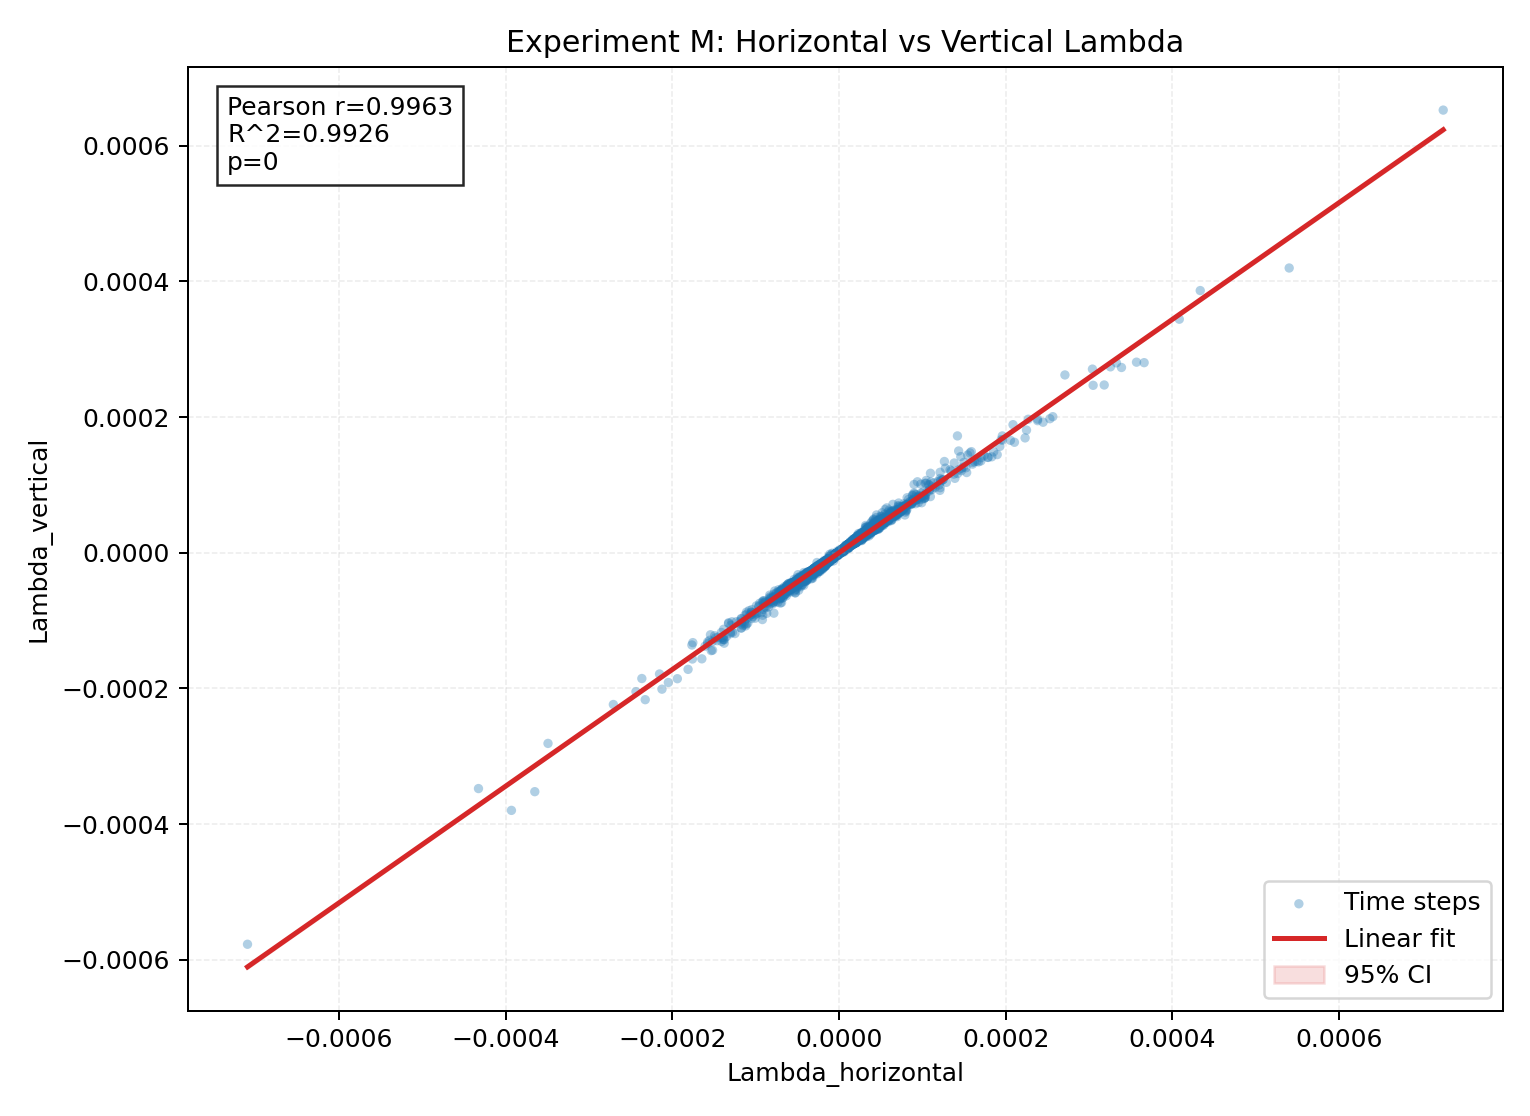
\includegraphics[width=\linewidth]{figures/plot_lambda_scatter.png}
\par\vspace{0.4em}
\small (a) Согласование предсказаний $\Lambda_{\mathrm{hor}}$ и $\Lambda_{\mathrm{vert}}$.
\end{minipage}\hfill
\begin{minipage}[t]{0.49\linewidth}
\centering
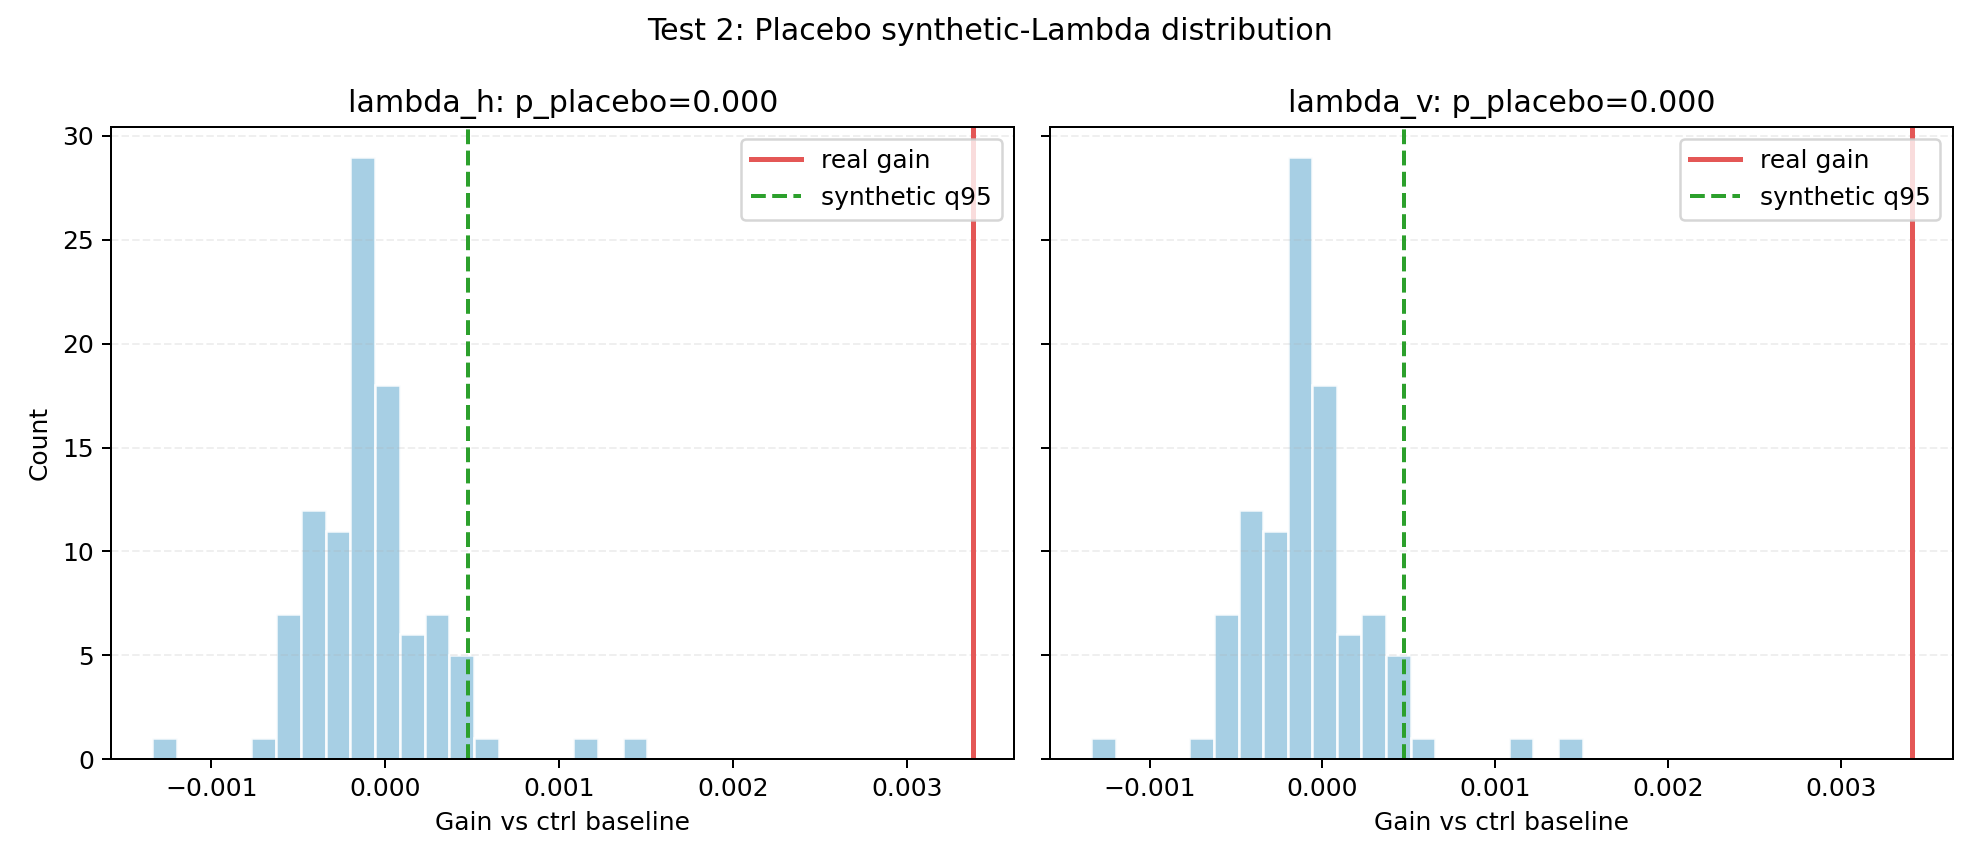
\includegraphics[width=\linewidth]{figures/plot_test2_placebo.png}
\par\vspace{0.4em}
\small (b) Распределение OOF-gain для плацебо-суррогатов.
\end{minipage}
\caption{Малый, но устойчивый макросигнал в блоках M1--M2. Этот блок фиксирует наблюдаемость и структурную согласованность; прямое локальное замыкание $\Lambda_b\sim\Pi_b$ проверяется отдельно в A15.}
\label{fig:macro_detectability}
\end{figure}

\subsection{Фальсификационные контроли необходимости \texorpdfstring{$\Lambda_{\mathrm{proxy}}$}{Lambda proxy} (M4)}

В блоке \texttt{experiment\_M\_lambda\_falsification\_tests} выполнены три адресных контроля необходимости \(\Lambda_{\mathrm{proxy}}\)
в той же OOF blocked-CV постановке.

\paragraph{S1: placebo-\(\mu\).}
При перестановке масштабных слоёв получено
\[
\Delta_{\mathrm{OOF}}(\Lambda_{\mathrm{real}})=0.003412,\qquad
\Delta_{\mathrm{OOF}}(\Lambda_{\mathrm{placebo\text{-}\mu}})=-0.002986,\qquad
p_{\mathrm{perm}}^{\mathrm{placebo}}=1.0.
\]
Разрушение межмасштабной структуры убирает наблюдаемый эффект и переводит gain в отрицательную область.

\paragraph{S2: \(F^{\mathrm{comm}}\)-контроль.}
Для коммутирующего контроля получено
\[
\Delta_{\mathrm{OOF}}(\Lambda_{\mathrm{comm}})=0,\qquad \beta_{\mathrm{comm}}=0,
\]
тогда как для \(\Lambda_{\mathrm{real}}\) сохраняется положительный gain.

\paragraph{S3: информационные критерии.}
При переходе \(\mathrm{ctrl}\to \mathrm{ctrl}+\Lambda_{\mathrm{real}}\) имеем
\[
\Delta \mathrm{AIC}=-13.202,\qquad \Delta \mathrm{BIC}=-6.817.
\]
В сумме эти тесты поддерживают более узкий, но и более надёжный вывод:
полезный сигнал связан именно с сохранённой межмасштабной структурой, а не с произвольной линейной добавкой.

\subsection{Предел наблюдаемости: суша/океан, термодинамический фон и пространственная диагностика}

Разбиение суша/океан фиксирует характерный парадокс наблюдаемости.
В постановке \texttt{residual\_full} над океаном сохраняется положительный и значимый сигнал
($\Delta_{\mathrm{OOF}}=0.001818$, $p=0.021$),
тогда как над сушей gain становится отрицательным
($-0.000491$, $p=0.879$).
Noise-probe показывает, что существенная часть этой разницы связана с более шумным членом $P-E$:
в варианте \texttt{residual\_no\_pe} land-gain практически исчезает
($-1.9\times10^{-5}$),
а при 24-часовом сглаживании \texttt{residual\_full\_roll4} восстановление сигнала наблюдается на обеих поверхностях
($0.001357$ над сушей и $0.004099$ над океаном).

Блок O1 добавляет ещё одно ограничение: на FT-слое классическое клаузиусово замыкание уже даёт
$R^2_{\mathrm{base}}=0.932165$,
а добавление $\Lambda_{\mathrm{proxy}}$ почти ничего не меняет
($R^2_{\mathrm{full}}=0.932161$, $\Delta R^2=-3.75\times10^{-6}$, $p_{\mathrm{perm}}=0.404$).
Соответственно, на макромасштабах текущего ERA5-разрешения межмасштабная поправка либо очень мала, либо подавлена термодинамическим фоном.

Блок O2 подтверждает ту же картину в пространственной форме:
\[
\mathrm{corr}(\mathrm{gain\_map},\mathrm{convective\_clim})=0.0317,\qquad
\max(\mathrm{gain\_map})=9.20\times10^{-4},
\]
а panel-контроль даёт лишь $3.42\times10^{-6}$ прироста.
Поэтому O1--O2 следует трактовать как диагностику предела наблюдаемости, а не как сильное подтверждение.

\begin{figure}[t]
\centering
\begin{minipage}[t]{0.49\linewidth}
\centering
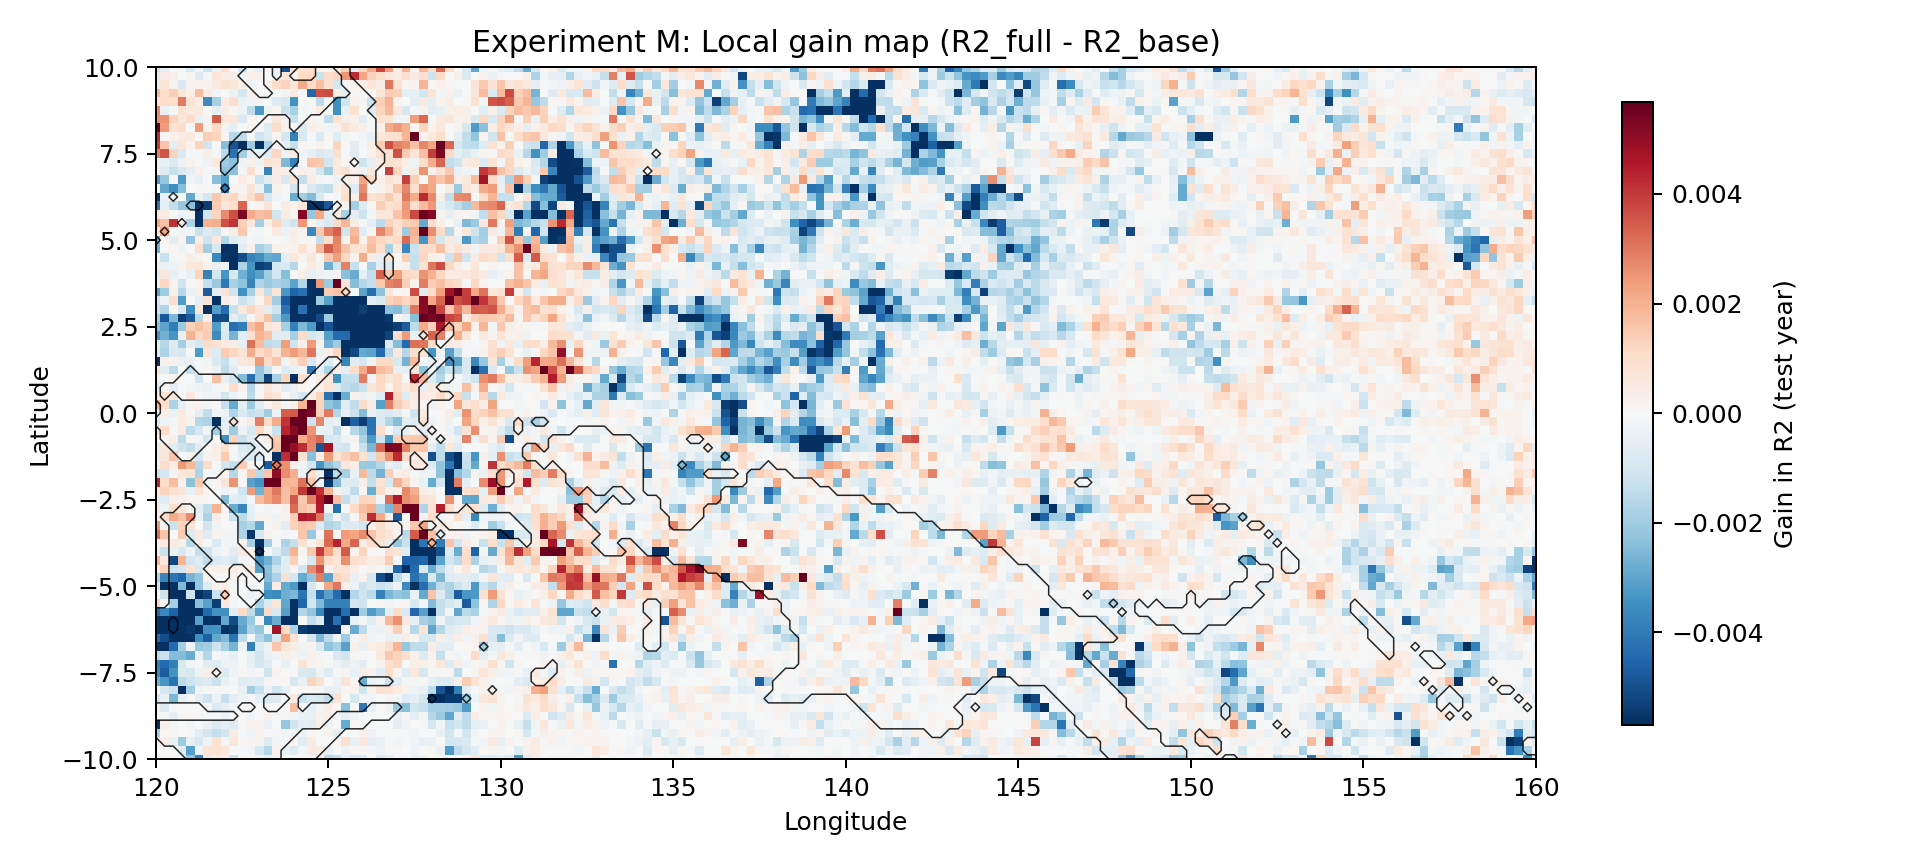
\includegraphics[width=\linewidth]{figures/plot_spatial_gain_map.png}
\par\vspace{0.4em}
\small (a) Локальная карта прироста качества $\Delta R^2$ (WPWP, береговая линия).
\end{minipage}\hfill
\begin{minipage}[t]{0.49\linewidth}
\centering
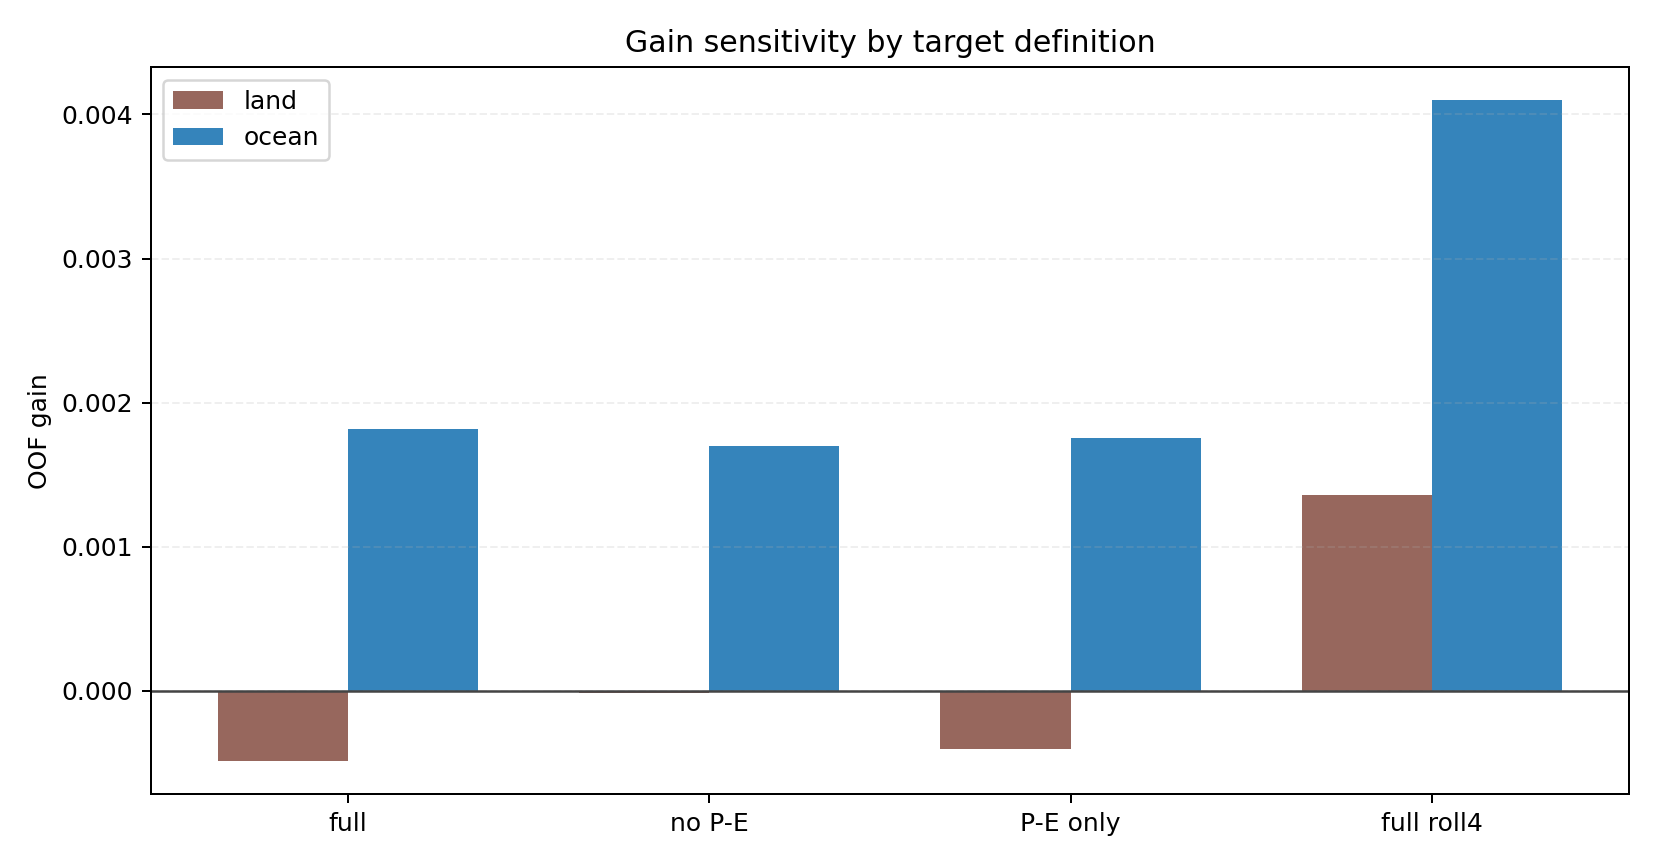
\includegraphics[width=\linewidth]{figures/plot_noise_probe_gains.png}
\par\vspace{0.4em}
\small (b) Медианный OOF-gain для сценариев \texttt{residual\_full}, \texttt{residual\_no\_pe} и \texttt{residual\_full\_roll4}.
\end{minipage}
\caption{Предел наблюдаемости в макроблоке: положительный океанический сигнал соседствует с режимом, близким к шумовому порогу, над сушей и с доминированием термодинамического базового приближения.}
\label{fig:macro_noise_limit}
\end{figure}

\subsection{Структурные суррогатные и хвостовые тесты: поддержка и отрицательные результаты}

Серия F5 усиливает основную M-постановку, но тоже не даёт права на чрезмерно сильные формулировки.
Главный критерий наблюдаемости проходит:
\(\Delta_{\mathrm{OOF}}=0.003412\ge 0.002\),
\(p_{\mathrm{perm}}=0.007092\),
\(\mathrm{strata\_positive\_frac}=1.0\).
Два независимых фрактальных суррогата (PSD-наклон и наклон вариограммы) дают положительную связь с \(\lvert\Lambda_{\mathrm{proxy}}\rvert\)
с корреляциями $0.300$ и $0.348$ соответственно, но согласие между самими суррогатами остаётся умеренным
(\(\mathrm{Spearman}=0.587\)).
Следовательно, F5 поддерживает структурную, но не окончательно уникальную интерпретацию сигнала.

Серия строгих хвостовых/SOC-тестов, напротив, в атмосфере оказывается отрицательной.
В F6b для глобального \(\lvert\Lambda_{\mathrm{local}}\rvert\) действительно наблюдается heavy-tail fit,
но показатель \(\alpha_{\mathrm{emp}}=3.3067\) выходит далеко за заранее объявленный диапазон SOC-универсальности $[1.5,2.0]$.
В F6c ни один кластер не проходит строгий corrected test, а в F6c-spatial не найдено ни одного spatial patch,
удовлетворяющего одновременно критериям по \(\alpha\), динамическому диапазону и LLR.
Именно поэтому в этой работе мы \emph{не утверждаем}, что атмосферный SOC подтверждён:
положительный модельный результат F6 и отрицательные атмосферные F6b/F6c/F6c-spatial должны читаться раздельно.

\subsection{A05: процессно-разрешённый межмасштабный мост и память на нижних слоях}

Центральный новый эмпирический вклад манускрипта --- серия A05, где тест переносится
с макроусреднённого ERA5-блока на процессно-разрешённую постановку на отдельных плитках и панелях.
Именно здесь формализм даёт наиболее содержательный эмпирический результат:
координата масштаба оказывается переносимой на разрежённых и плотных панелях, но на самом тонком масштабе требуется память.

\begin{table}[t]
\centering
\caption{Сводка A05.R1--A05.R6. Финальная лестница памяти читается как R3$\to$R6: перенос на плотную панель ломает $l=8$, диагностика локализует проблему в чувствительности тонкомасштабного режима, минимальное замыкание с памятью восстанавливает сигнал, а полная GKSL/CPTP-ветка показывает, что восстановление не является частным техническим артефактом.}
\label{tab:A05_summary}
\small
\begin{tabular}{@{}p{1.4cm}p{4.9cm}p{6.0cm}@{}}
\toprule
Блок & Что тестируется & Итог \\
\midrule
A05.R1 & Каскад заполнения $l\to 2l$ на разрежённой панели & ALL: $\mathrm{mae\_gain}=5.10\times10^{-5}$, $\mathrm{R}^2$-gain $=0.0220$; масштабы $l=8,16$ проходят с $\mathrm{perm\_p}=0.02$, а $l=32$ остаётся пограничным. \\
A05.R2 & Калибровка некоммутирующего моста матрицы плотности C009 & Выбран базовый C009: overall $\mathrm{mae\_gain}=7.43\times10^{-6}$, $\mathrm{R}^2$-gain $=0.003392$; все масштабы проходят на разрежённой панели. \\
A05.R3 & Перенос C009 на плотную внутрисобытийную выборку & ALL остаётся положительным ($3.10\times10^{-7}$), $l=16,32$ проходят, но $l=8$ деградирует: $\mathrm{perm\_p}=0.80$, PASS\_ALL=False. \\
A05.R4 & Узкая диагностика провала на $l=8$ & Контроли по совпадающим событиям, разложение по операторам и режимное расщепление показывают, что проблема связана с чувствительностью тонкомасштабного режима, а не с составом пула событий; combo-check даёт $\mathrm{mae\_gain}=6.98\times10^{-6}$ и $\mathrm{perm\_p}=0.02$, но остаётся только диагностикой. \\
A05.R5 & Ретардированная память матрицы плотности поверх фиксированного C009 & Конфигурация M001 ($\eta=0.8$, $\tau=0.75$) восстанавливает $l=8$: $\mathrm{mae\_gain}=1.22\times10^{-6}$, $\mathrm{perm\_p}=0.02$, event-positive fraction $=0.9375$; all-scale PASS\_ALL=True. \\
A05.R6 & Полная GKSL/CPTP-динамика памяти поверх фиксированного C009 & Конфигурация G001 даёт $l=8$: $\mathrm{mae\_gain}=2.27\times10^{-6}$, $\mathrm{perm\_p}=0.02$, event-positive fraction $=0.9375$; all-scale PASS\_ALL=True, а proxy нарушения CPTP равен $8.88\times10^{-16}$. \\
\bottomrule
\end{tabular}
\end{table}

Интерпретация этой последовательности важнее отдельных метрик.
R1--R2 показывают, что межмасштабный мост в процессно-разрешённой постановке вообще детектируется и переносится.
Финальная лестница памяти затем читается как R3$\to$R6.
R3 показывает, что при переходе к плотной внутрисобытийной выборке общий сигнал не исчезает, но именно мгновенное описание на тончайшем масштабе ломается на $l=8$.
R4 снимает простое объяснение через состав пула событий: контроли по совпадающим событиям оставляют провал на месте и указывают на чувствительность тонкомасштабного режима.
R5 показывает, что минимального замыкания с памятью уже достаточно, чтобы восстановить переносимость без удаления квадратичного канала и без снижения стандартного порога активности.
R6 повторяет это восстановление в более строгой полной GKSL/CPTP-постановке и тем самым показывает, что эффект не сводится к специально подобранному суррогатному рецепту.

\clearpage
\begin{figure}[H]
\centering
\begin{minipage}[t]{0.92\linewidth}
\centering
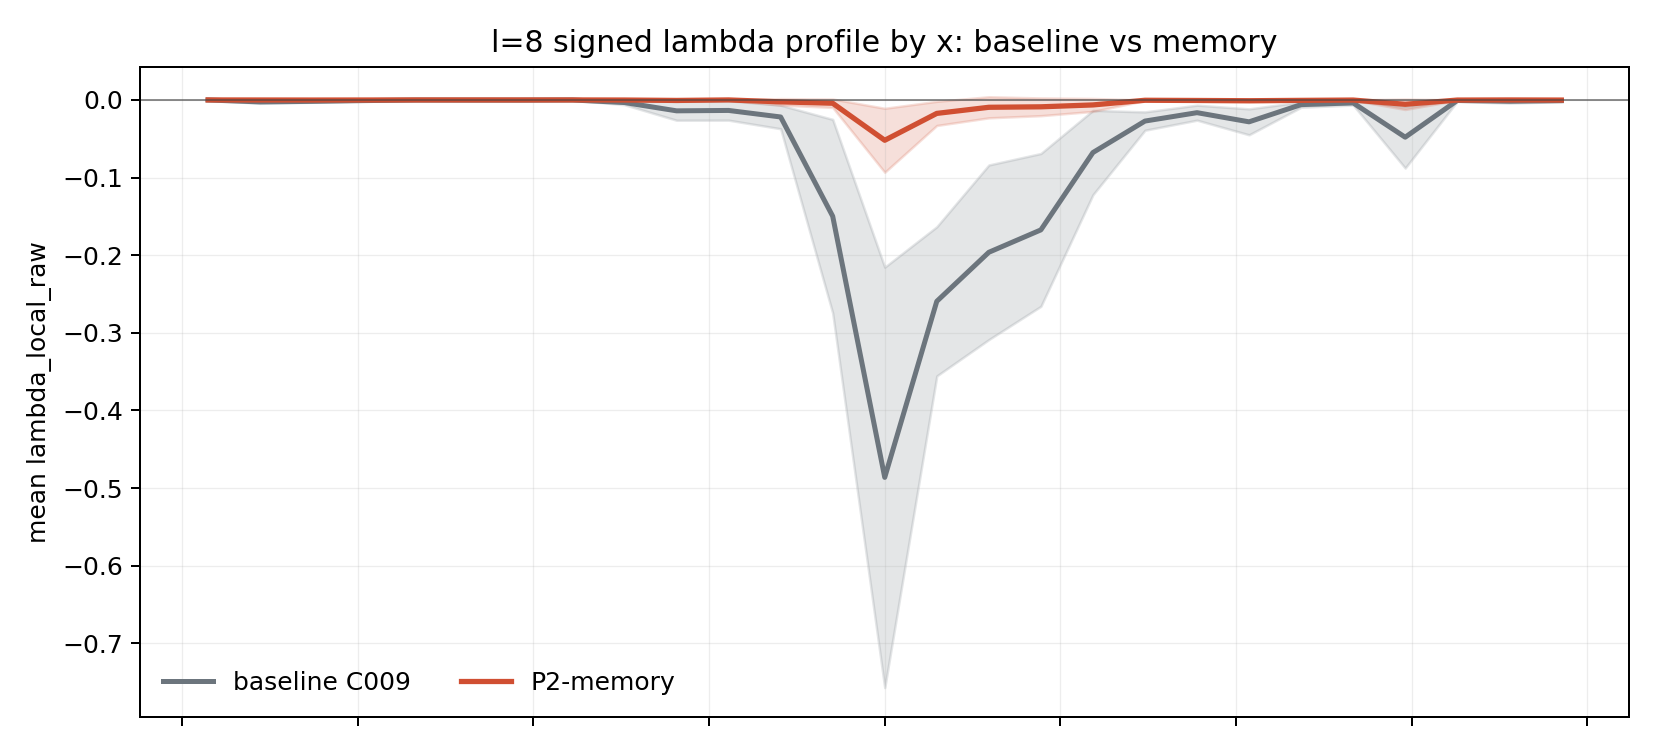
\includegraphics[width=\linewidth]{figures/a05_r5_l8_lambda_profile_baseline_vs_memory.png}
\par\vspace{0.4em}
\small (a) На $l=8$ мост с памятью ослабляет отрицательный провал и поднимает signed $\lambda(x)$ относительно базовой плотной схемы.
\end{minipage}

\par\vspace{0.9em}

\begin{minipage}[t]{0.92\linewidth}
\centering
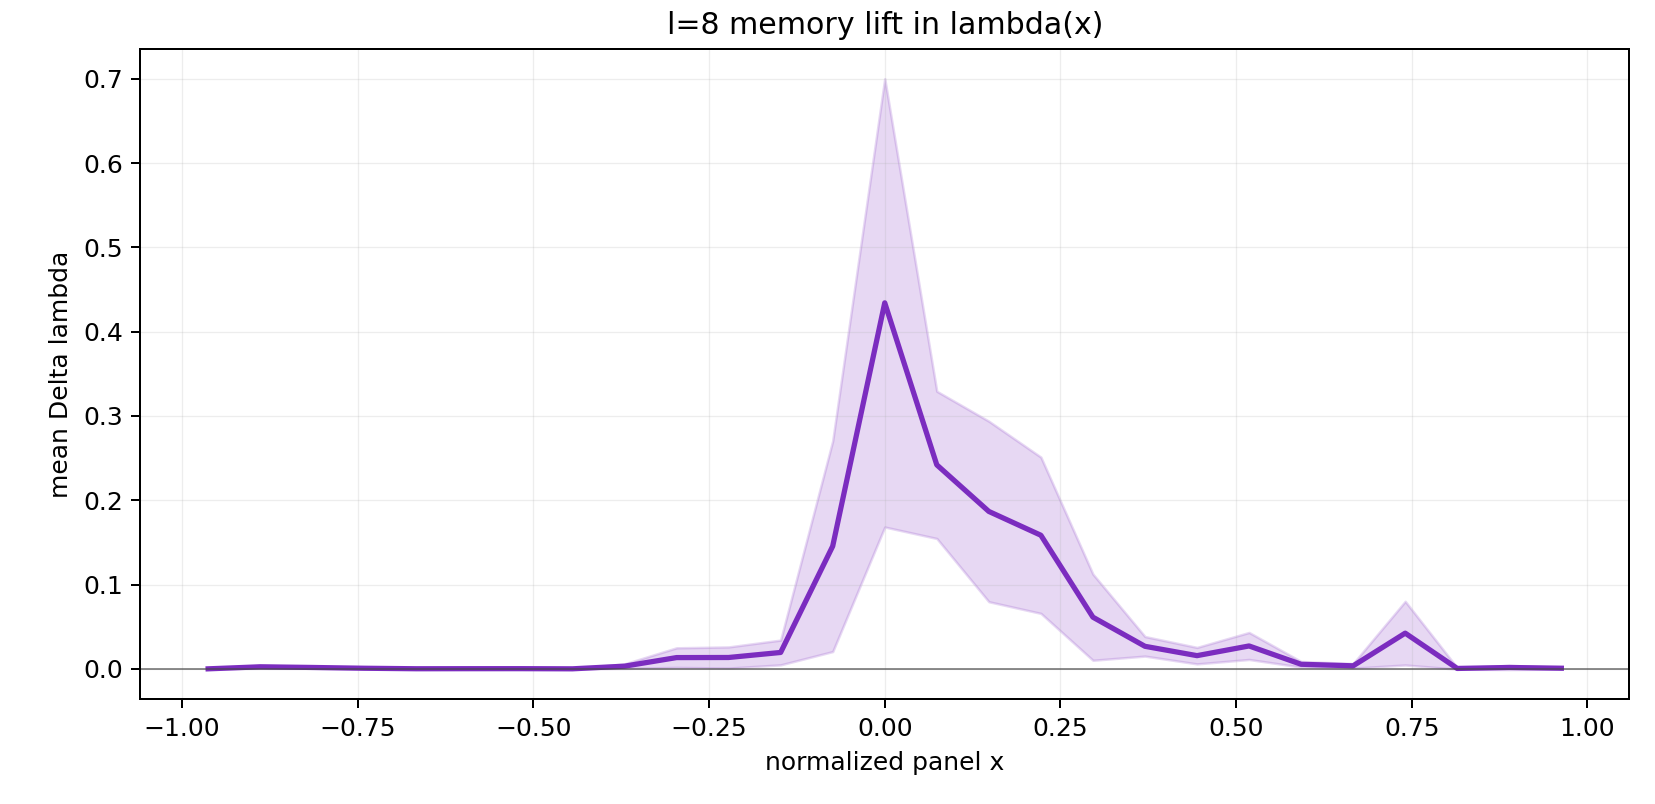
\includegraphics[width=\linewidth]{figures/a05_r5_l8_memory_lift_by_x.png}
\par\vspace{0.4em}
\small (b) Прибавка $\Delta \lambda(x)$ локализована в центральных $x$-бинах и не сводится к равномерному аддитивному сдвигу.
\end{minipage}
\caption{A05.R5: ретардированная память матрицы плотности как минимальное, максимально близкое к формализму замыкание тончайшего режима. Эта ступень трактуется как \emph{минимальный ретардированный суррогат}; более строгая GKSL/CPTP-проверка R6 обсуждается непосредственно в тексте ниже.}
\label{fig:A05_memory}
\end{figure}

R6 завершает эту ветку уже в более строгой физической постановке. В полной GKSL/CPTP-динамике памяти
конфигурация G001 даёт для $l=8$ $\mathrm{mae\_gain}=2.27\times10^{-6}$ при $\mathrm{perm\_p}=0.02$,
сохраняет all-scale PASS\_ALL=True и при этом оставляет proxy нарушения CPTP на уровне $8.88\times10^{-16}$.
Именно это переводит R5 из удачного минимального суррогата в часть более общей воспроизводимой ветви памяти.

Именно A05 позволяет сформулировать два центральных эмпирических тезиса работы в сдержанной форме.
Во-первых, координата масштаба над фиксированным $x$ оказывается операционально осмысленной и переносимой при модуляции.
Во-вторых, на самых мелких масштабах чисто марковское мгновенное описание оказывается недостаточным:
для восстановления переноса требуется память, причём этот вывод удерживается и в минимальном суррогате R5, и в более строгой GKSL/CPTP-реализации R6.

\subsection[A15: локальный тест Lambda-b--Pi-b замыкания]{A15: локальный тест Lambda-b--Pi-b замыкания (``Эйнштейн в атмосферном столбе'')}

После макро- и процессно-разрешённых блоков выполняется прямой локальный тест
операционального \(\Lambda_b\sim\Pi_b\)-замыкания на ERA5.
Постановка A15 использует вектор ветра \((u,v)\), масштабные полосы
\([50,100,200,400,800,1600,3200]\) км, скользящее окно \(W=20\),
операторную реконструкцию \(\rho_\mu\), \(G_{\mathrm{fwd/back}}\), \(F\), \(\Lambda_b=\Re\Tr(F_b\rho_b)\)
и прокси спектрального потока энергии
\[
\Pi_b(t)=\left\langle |k|\,E(k,t)\right\rangle_{k\in b},
\qquad
E(k,t):=\frac{|\hat u(k,t)|^2+|\hat v(k,t)|^2}{2}.
\]
На базовом окне ERA5
\(2017\text{-}01\text{-}01\;00{:}00{:}00 \ldots 2017\text{-}03\text{-}31\;18{:}00{:}00\)
(360 шагов, 6-часовая дискретизация)
получено:
\[
R^2_{\mathrm{binned,inertial}}=0.520,\qquad
\beta_{\mathrm{inertial}}>0,\qquad
p_{\mathrm{slope}}=0.008.
\]
Одновременно зона подпитки демонстрирует инверсию/ослабление наклона
(\(R^2_{\mathrm{binned}}=0.179\), отрицательный коэффициент наклона),
а зона диссипации показывает падение качества
(\(R^2_{\mathrm{binned}}=0.371\)).
Критерии успешности ERA для A15 задавались заранее как
\(R^2_{\mathrm{binned,inertial}}\ge 0.40\), положительный и значимый коэффициент наклона
в инерционном подинтервале, а также контролируемый распад связи на краях подпитки/диссипации;
в базовом окне они выполнены (\texttt{PASS\_ALL=True}).
Таким образом, на реальных атмосферных данных фиксируется именно тот режимный профиль,
который ожидается для локального масштабного замыкания:
работа в инерционном подинтервале и контролируемый распад связи на краях каскада.
Это даёт эмпирическую поддержку тому, что калибровочно-инвариантная полосовая величина \(\Lambda_b\),
построенная из кривизны связности и состояния, ведёт себя как геометрическая прокси-величина,
согласованная со спектральным потоком энергии в инерционном интервале.
\begin{figure}[H]
\centering
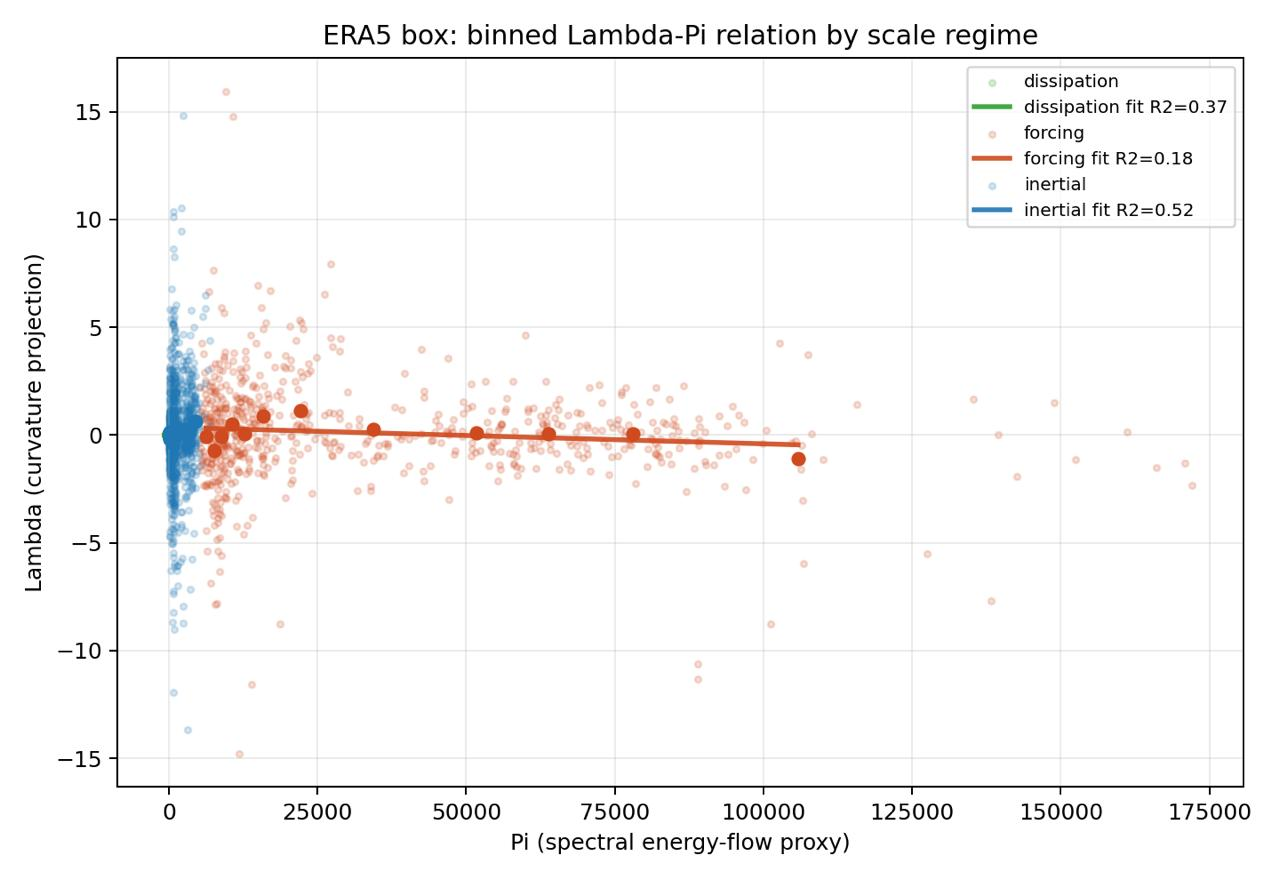
\includegraphics[width=0.9\linewidth]{figures/a15_lambda_vs_pi_regimes.png}
\caption{A15: связь \(\Lambda_b\sim\Pi_b\) по режимам в атмосферном столбе ERA5. В инерционном подинтервале наблюдается устойчивая положительная зависимость, тогда как на краях каскада (зона подпитки и зона диссипации) связь закономерно ослабевает или меняет знак.}
\label{fig:a15_lambda_pi_regimes}
\end{figure}

\subsection{Предел локального переноса и тесты физически соседнего окружения}

Строгий хронологический тест A11, в котором проверялся перенос добавки $\Phi$ поверх $\Lambda_{\mathrm{proxy}}$ в постановке обучение$\le 2019 \rightarrow$ тест $2020 \rightarrow$ внешний контроль $2021$, даёт отрицательный результат. Для контрольного 2020 года получаем $\Delta_{\Lambda_{\mathrm{proxy}},\mathrm{ctrl}}=-0.002240$ при $p=0.4055$, а добавка $\Phi$ поверх $\Lambda_{\mathrm{proxy}}$ даёт лишь $\Delta_{\Phi,\Lambda_{\mathrm{proxy}}}=-0.000067$ при $p=0.3810$; на внешнем 2021 остаётся $\Delta_{\Phi,\Lambda_{\mathrm{proxy}}}=-0.000023$ при $p=0.3350$. Иными словами, перенос локального замыкания на одной плитке не демонстрирует устойчивого обобщения в строгой постановке прогноза на год вперёд.

Блок A12 снимает это ограничение, вводя физически соседнее граничное окружение при оценке только по внутреннему ядру. Здесь модель \texttt{ERA\_window} резко превосходит \texttt{ERA\_core}: выигрыш составляет $0.136707$ на тесте 2020 и $0.092229$ на внешнем контроле 2021, в обоих случаях при $p=0.0005$. Прибавки от $\Phi_H$ и $\Lambda_H$ поверх этого окна малы, поэтому основной эффект связан именно с наличием физически примыкающего окружения.

Блок A13 уточняет этот вывод сканированием ширины граничного кольца. При $w=0$ выигрыш исчезает, а максимум достигается при $w=4$: $0.151703$ на тесте и $0.156626$ на внешнем контроле; при $w=6,8,10$ эффект остаётся положительным, но последовательно ослабевает. Следовательно, речь идёт не о пользе произвольно расширяемого набора признаков, а о локальном и немонотонном масштабе граничного взаимодействия.

Блок A14 завершает серию фальсификационным сравнением физически примыкающего окружения с удалённым и смещённым. При фиксированном $w=4$ локальное окружение уверенно превосходит оба контроля: \texttt{local} даёт $0.151703/0.156626$, тогда как \texttt{remote} --- $0.097182/0.058412$, а \texttt{misaligned} --- $0.073343/0.059724$ на тесте и внешнем контроле соответственно. Это означает, что для атмосферного переноса существенно именно физически соседнее окружение, а не любой дополнительный внешний сигнал.

\paragraph{Пределы интерпретации атмосферного блока.}
Текущие атмосферные данные слишком грубы, чтобы идентифицировать полную внутреннюю структуру объекта $\Lambda_{\mathrm{matter}}$ и его полосовых проекций из формальной модели.
Однако их достаточно, чтобы проверить, сохраняются ли предсказанные формализмом наблюдаемые паттерны после огрубления и измерительных ограничений, включая прямую связь $\Lambda_b\sim\Pi_b$ в инерционном интервале.
Самые сильные эмпирические результаты этого раздела теперь включают: (i) прямую локальную проверку \(\Lambda_b\sim\Pi_b\) в A15, (ii) роль памяти в A05.R5--R6, (iii) зависимость от физически соседнего граничного окружения в A12--A14. Термодинамические и SOC-связанные сигналы остаются вторичными и ограниченными по силе вывода.

\begin{table}[H]
\centering
\caption{Синтетическая сводка блока A12--A14.}
\label{tab:A12_A14_summary}
\small
\begin{tabular}{@{}p{2.8cm}p{3.9cm}p{4.0cm}p{4.0cm}@{}}
\toprule
Вопрос & Протокол & Основной результат & Интерпретация \\
\midrule
A12: нужно ли физически соседнее окружение? & Оценка по внутреннему ядру при добавлении граничного кольца вокруг него; строгий перенос обучение$\le 2019 \rightarrow 2020 \rightarrow 2021$. & \texttt{ERA\_window} даёт $0.136707/0.092229$ относительно \texttt{ERA\_core}; добавки $\Phi_H$ и $\Lambda_H$ малы. & Ключевой выигрыш создаёт само физически примыкающее окружение. \\
A13: какова характерная ширина окружения? & Фиксированная постановка ядра и сканирование ширин $w\in\{0,4,6,8,10\}$. & Максимум достигается при $w=4$: $0.151703/0.156626$; при больших $w$ эффект насыщается и ослабевает. & Граничный эффект локален и немонотонен по ширине. \\
A14: важно ли именно соседнее окружение? & При $w=4$ сравниваются локальное, удалённое и смещённое окружения при одинаковой метрике ядра. & \texttt{local} превосходит \texttt{remote} и \texttt{misaligned}: $0.151703/0.156626$ против $0.097182/0.058412$ и $0.073343/0.059724$. & Существенно именно физически соседнее окружение, а не произвольная внешняя информация. \\
\bottomrule
\end{tabular}
\end{table}

Итоговая логика раздела такова: A11--A14 задают границу переносимости локальной редукции и показывают решающую роль физически соседнего окружения, а A15 даёт самый жёсткий и прямой эмпирический результат всей атмосферной части --- локальную проверку \(\Lambda_b\sim\Pi_b\) в инерционном интервале ERA5 (см.\ \cref{fig:a15_lambda_pi_regimes}).

\paragraph{Воспроизводимость (эмпирический блок).}
Канонический набор core-скриптов для эмпирического блока опубликован в активном релизе:
\url{https://github.com/Theclimateguy/Shroedinger/releases/tag/v2.1}.
Тяжёлые промежуточные/итоговые артефакты и continuation-прогоны (A05.R* и A07.R*) сохраняются как отдельные runtime-выгрузки и не входят в компактный пакет по умолчанию.

% =========================================================
\section{Обсуждение: что поддержано, что остаётся гипотезой}
\label{sec:discussion}

\paragraph{Что поддержано текущими данными.}
На уровне модельной валидации формализм выглядит внутренне согласованным:
калибровочные инварианты устойчивы, баланс на $(t,x,\mu)$ замыкается,
а блоки F1--F6 вместе с T20 показывают, что внутри одного численного класса можно последовательно связать балансный режим,
масштабную ковариантность, фрактальные прокси, голономию и модельный SOC.
На уровне атмосферы поддержка также стала более прямой:
M1--M4 дают слабый и воспроизводимый структурный сигнал в задаче замыкания,
а A05.R3--R6 даёт завершённую лестницу памяти: перенос на плотную панель ломает именно $l=8$,
диагностика привязывает этот провал к чувствительности тонкомасштабного режима, минимальное замыкание с памятью восстанавливает сигнал,
и более строгая GKSL/CPTP-реализация подтверждает, что восстановление не является частным техническим артефактом.
Ключевое дополнение A15 даёт прямую эмпирическую поддержку \(\Lambda_b\sim\Pi_b\) в инерционном диапазоне ERA5
(\(R^2_{\mathrm{binned}}=0.520\), \(p=0.008\)) при ожидаемом распаде связи в диапазонах подпитки/диссипации.

\paragraph{Граница локальной атмосферной редукции.}
A05.R6 показывает, что физика памяти на тончайшем масштабе работоспособна в процессно-разрешённой постановке: восстановление удерживается не только в минимальном суррогате, но и в полной GKSL/CPTP-динамике. В то же время блок A11--A14 показывает границу применимости более жёсткой локальной атмосферной редукции: перенос на одной плитке не обобщается устойчиво в постановке на год вперёд, тогда как физически соседнее окружение даёт крупный и воспроизводимый выигрыш. A15 завершает эту картину как наиболее твёрдое эмпирическое основание: локальное $\Lambda_b\sim\Pi_b$-замыкание поддержано в режиме локальной ячейки, но остаётся режимно-зависимым при смене окна и внешнего динамического режима.

Следующий естественный шаг поэтому состоит не в ещё одной локальной абляции, а в построении более полной атмосферной модели открытой системы, где окружение локальной подсистемы задаётся явно. На уровне постановки это указывает на необходимость перехода от одиночной плитки к квазиглобальной или, в пределе, целостной атмосферной конфигурации с контролируемым межмасштабным и межобластным обменом.

\paragraph{Что пока не поддержано.}
Те же данные не позволяют делать более сильные выводы.
Мы не установили физический статус $\Lambda_{\mathrm{matter}}$ как фундаментальной константы;
она остаётся эффективным источником и диагностическим прокси-членом.
Мы не вывели термодинамическое замыкание по первым принципам для всей реальной атмосферы:
O1--O2 и окно-зависимость A15 показывают, что вне режима локальной ячейки и без явного учёта режима
сигнал может быть существенно ослаблен.
Наконец, мы не подтверждаем универсальный атмосферный SOC-режим:
строгие хвостовые и кластерные тесты F6b/F6c/F6c-spatial остаются отрицательными.

\paragraph{Операциональные находки и сильные интерпретации --- не одно и то же.}
Наиболее надёжный операциональный результат работы состоит в том, что координата масштаба полезна как переменная описания
и что на нижних слоях требуется память, а на атмосферном уровне локальная подсистема чувствительна к физически соседнему окружению.
R6 усиливает первый вывод, а A12--A14 --- второй.
Но это всё ещё не тождественно утверждению о полной немарковской теории природы, не доказывает универсальную 5D-геометрию
и не снимает необходимость отдельного вывода динамики с памятью и явной модели окружения.
Именно это различие мы считаем принципиальным для честного позиционирования результата.

\paragraph{Связь с близкими направлениями.}
Предлагаемая рамка естественно соприкасается с RG-геометрией и локальным RG
\cite{Zamolodchikov1986Irreversibility,Osborn1991LocalRG,CotlerRezchikov2023RGOptimalTransport},
с информационной геометрией и голономией квантовых каналов
\cite{Amari2016InformationGeometry,Uhlmann1986QuantumHolonomy,KultAbergSjoqvist2008HolonomyChannels},
а также с термодинамической гравитацией в духе Джейкобсона
\cite{Jacobson1995EinsteinEOS,ElingGuedensJacobson2009NonEq}.
Отличие нашей работы в том, что эти идеи используются как рабочие ориентиры для проверяемой программы,
а не как уже замкнутый фундаментальный вывод.

\section{Ограничения и дальнейшая работа}
\label{sec:limitations}

В рамках заявленного уровня (локальное масштабно-термодинамическое замыкание в ячейке) теория закрыта в операциональном смысле: T20 и A15 дают прямую эмпирическую поддержку связи \(\Lambda_b\sim\Pi_b\) в инерционном интервале.
При выходе за этот уровень сохраняются открытые вопросы.
Более строго, внутреннее геометрическое ядро масштабной ячейки может быть замкнуто как локальная вариационная модель: заданное поле проектора \(P_*(s,\mu)\) можно получить из CP1/O(3)-типа действия на двумерной базе \((s,\mu)\), после чего связность \(A_i\), кривизна \(F_{ij}\) и локальный объект вида \(\mathrm{Tr}(\rho F)\) уже не являются свободными величинами. Однако это не является полным фундаментальным выводом: такая внутренняя ячейка не фиксирует сама по себе абсолютную шкалу KMS-релаксации, нормировку \(T_{\alpha\beta}^{\mathrm{scale}}\) при вариации по метрике и физическую карту источника \(\rho_{\mathrm{phys}}\mapsto(s,\Delta,\beta)\). Поэтому все утверждения статьи следует читать как локальное операциональное и модельно-геометрическое замыкание, а не как завершённую теорию гравитационного источника.
Ветка памяти в A05 теперь включает и минимальный суррогат R5, и более строгую GKSL/CPTP-реализацию R6. Это существенно усиливает физическую состоятельность результата, но всё ещё не заменяет общего вывода немарковской динамики с историческим ядром, выведенным по первым принципам.
Термодинамический блок в локальном режиме поддержан эмпирически, но это не эквивалентно универсальному выводу по первым принципам для полной атмосферы или общей квантово-полевой системы.
Атмосферный сигнал остаётся режимно-зависимым. Помимо WPWP/ERA5 и канонической A05-панели, строгий блок A11--A14 показывает, что перенос локального замыкания на одной плитке неустойчив, а воспроизводимый выигрыш возникает лишь при явном учёте физически соседнего окружения. Frozen-extensions A07.R1--A07.R5 (см. \hyperref[sec:appendix:atmo]{Приложение~A.3}) усиливают этот вывод: в независимых расширениях часть прогонов остаётся отрицательной или пограничной. Это подчёркивает необходимость независимых географических и сезонных повторов без ретюнинга.
Для более сильных выводов нужны данные следующего класса: более плотные процессно-разрешённые панели, LES/CRM-уровень для прямой проверки термодинамики на самых мелких масштабах, а также независимые регионы и сезоны с заранее зафиксированным протоколом.
Физический статус $\Lambda_{\mathrm{matter}}$, универсальность термодинамического замыкания и возможная связь с более широкой фундаментальной теорией остаются открытыми.


\section{Заключение}
\label{sec:conclusion}

В работе предложен формализм геометрии масштаба на расширенной базе $(x,t,\mu)$ с ковариантной динамикой и согласованным огрублением.
В контролируемых модельных экспериментах формализм проходит внутреннюю валидацию (калибровочная согласованность, баланс, мостовые и структурные проверки) и приводит к конструктивно определённой наблюдаемой $\Lambda_{\mathrm{matter}}$ и её полосовой версии $\Lambda_b$.

На модельном этапе T20 в инерционном диапазоне наблюдается устойчивая связь \(\Lambda_b\sim\Pi_b\), а в атмосферном блоке A15 получена эмпирическая поддержка той же локальной зависимости на данных ERA5. Этот результат согласуется с термодинамической интерпретацией геометрического замыкания, но относится именно к контролируемому режиму локальной ячейки.

Наиболее сильные эмпирические результаты статьи относятся к трём узлам программы: роли памяти на тонких масштабах (A05.R5--R6), локальному $\Lambda_b\sim\Pi_b$-замыканию (T20/A15) и физически соседнему граничному окружению (A12--A14). Вместе они задают не универсальную теорию, а согласованный и воспроизводимый операциональный набор следствий формализма.

Полученная картина поддерживает термодинамико-геометрическое чтение модели, но не снимает открытых вопросов о фундаментальном статусе $\Lambda_{\mathrm{matter}}$, универсальности замыкания вне локальной ячейки и выводе памяти по первым принципам.

Итоговая логика рукописи остаётся иерархической:
формализм, затем контролируемая валидация, затем эмпирические тесты грубых следствий, затем границы применимости и дальнейшие шаги.

% =========================================================
\appendix
\newpage

\phantomsection
\section*{Приложение C. Глоссарий терминов и сокращений}
\addcontentsline{toc}{section}{Приложение C. Глоссарий терминов и сокращений}
\label{sec:appendix:glossary}

\subsection*{C.1 Сокращения}

\begin{table}[H]
\centering
\caption{Основные сокращения в тексте.}
\label{tab:appendix_c_abbr}
\small
\begin{tabular}{@{}p{2.8cm}p{11.2cm}@{}}
\toprule
Сокращение & Краткое пояснение \\
\midrule
ERA5 & Глобальный реанализ атмосферы ECMWF (многолетний согласованный архив полей атмосферы). \\
WPWP & Пилотная постановка по тропическому влагобюджету в рамках текущего набора экспериментов. \\
OOF & \textit{Out-of-fold}: проверка на фрагментах данных, не участвовавших в обучении на данном шаге. \\
GKSL & Уравнение открытой квантовой динамики (Горини--Коссаковский--Сударшан--Линдблад). \\
CPTP & Класс отображений, сохраняющих физичность состояния: полная положительность и сохранение следа. \\
SOC & Самоорганизованная критичность (режим степенных хвостов в системах с медленным подводом и резкими сбросами). \\
RG & Ренормгрупповая эволюция по масштабу. \\
LES/CRM & Высокодетальные классы атмосферного моделирования (крупновихревое и облако-разрешающее). \\
MRMS/GOES & Наборы наблюдений высокого разрешения (радарный и спутниковый каналы). \\
\bottomrule
\end{tabular}
\end{table}

\subsection*{C.2 Ключевые термины простым языком}

\begin{table}[H]
\centering
\caption{Термины, важные для междисциплинарного чтения.}
\label{tab:appendix_c_terms}
\small
\begin{tabular}{@{}p{3.6cm}p{10.4cm}@{}}
\toprule
Термин & Пояснение без узкоспециальных деталей \\
\midrule
Гамильтониан $H$ & Оператор, задающий ``правило хода'' системы во времени: какие состояния и как быстро меняются. \\
Гильбертово пространство & Линейное пространство состояний с внутренним произведением; в работе это ``контейнер'' для состояния на каждом масштабе. \\
Гильбертово расслоение & Семейство таких пространств над точками $(x,t,\mu)$: у каждого положения и масштаба свой слой состояний. \\
Матрица плотности $\rho$ & Способ описывать не только ``чистое'' состояние, но и смесь состояний и неполную информацию о системе. \\
Когерентность & Недиагональные элементы $\rho$; характеризуют согласованность фаз между компонентами состояния. \\
Калибровочная связность $A_M$ & Правило, как согласованно переносить состояния и операторы между соседними точками/масштабами; задаёт ``геометрию переноса''. \\
Калибровочная инвариантность & Требование, чтобы физический вывод не зависел от выбранного локального базиса (``системы координат'' во внутреннем пространстве). \\
Связность по масштабу $A_\mu$ & Оператор, описывающий перенос информации между соседними масштабами. \\
Кривизна $F_{\mu\nu}$ & Мера некоммутативности переносов; из неё строятся инвариантные диагностические скаляры. \\
Голономия & Интегральный эффект переноса по замкнутому контуру: после обхода контура состояние может вернуться с нетривиальным ``поворотом''. \\
Причинный алмаз & Локальная область пространства-времени, задаваемая пересечением будущего и прошлого световых конусов; используется как малый домен для локальных термодинамических оценок. \\
Локальный горизонт & Граница причинной доступности для выбранного локального наблюдателя; через неё в термодинамическом маршруте учитывается поток энергии. \\
Модульный генератор & Оператор $K=-\log\rho_{\mathrm{ref}}$, кодирующий структуру локального референс-состояния; в малом алмазе связан с буст-потоком. \\
Детальный баланс & Условие согласованности диссипативной динамики с локальным референс-состоянием; обеспечивает неотрицательное производство энтропии. \\
Голографическое обрезание (экран) & Практическое ограничение числа степеней свободы по ``пограничному'' правилу, чтобы контролировать рост размерности модели при сохранении основной структуры. \\
Огрубление масштаба & Переход от более детального описания к более крупному (усреднённому) без нарушения физической корректности состояния. \\
Марковский предел & Приближение без ``памяти'' о прошлом: следующее состояние зависит только от текущего. \\
Память (немарковость) & Ситуация, когда прошлые состояния заметно влияют на текущую динамику. \\
Фальсификационный контроль & Специальный тест, который должен разрушить эффект, если тот вызван артефактом, а не структурой модели. \\
Граничное окружение (ореол) & Физически соседняя область вокруг ядра прогноза; в статье это ключевой фактор улучшения замыкания. \\
\bottomrule
\end{tabular}
\end{table}

\phantomsection
\section*{Приложение T. Теоретическая и модельная валидация}
\addcontentsline{toc}{section}{Приложение T. Теоретическая и модельная валидация}
\label{sec:appendix:toy}

\subsection*{T.0 Полный вывод эйнштейновского термодинамического маршрута}
\label{sec:appendix:einstein_full}

\paragraph{Статус этого приложения.}
Ниже дан полный технический маршрут, который в основном тексте был сокращён до итоговой формулы.
Этот путь сохраняется как интерпретационный и проверочный инструмент согласованности формализма,
но не используется как главный эмпирический вывод.

\paragraph{Шаг 1: модульный генератор локального референс-состояния.}
Для малого причинного алмаза $\Omega$ задаём
\begin{equation}\label{eq:app_modular_state}
\hat\rho_{\Omega}^{\mathrm{ref}}
=
Z_\Omega^{-1}\exp\!\left(-\hat K_{\Omega}^{\mathrm{mod}}\right),
\qquad
\hat K_{\Omega}^{\mathrm{mod}}:=-\log \hat\rho_{\Omega}^{\mathrm{ref}}.
\end{equation}
В дискретной реализации:
\begin{equation}\label{eq:app_modular_discrete}
\hat K_{\Omega}^{\mathrm{mod}}
=
\sum_{i\in\Omega}\kappa_i h_i,
\qquad
\kappa_i=-\log p_i^{\mathrm{ref}}.
\end{equation}

\paragraph{Шаг 2: локальный ``первый закон'' из относительной энтропии.}
Используя (A1)--(A3) и \cref{eq:entropy_production_local}, получаем
\begin{equation}\label{eq:app_firstlaw_mod}
\delta S_{\mathrm{hor}}
=
\delta\!\left\langle K_{\Omega}^{\mathrm{mod}}\right\rangle
+O(\varepsilon^2).
\end{equation}
Идентификация потока энергии через баланс \cref{eq:balance} приводит к локальной форме
\begin{equation}\label{eq:app_clausius}
T_\ast\,\dd S_{\mathrm{hor}}
=
\delta Q_{\mathrm{in}}
=
\int_{\partial\Omega}T_{ab}\chi^a\,\dd\Sigma^b
+O(\varepsilon^2).
\end{equation}

\paragraph{Шаг 3: предел малого алмаза и буст-генератор.}
При (A5) модульный поток асимптотически переходит в локальный буст-поток:
\begin{equation}\label{eq:app_boost_limit}
\hat K_{\Omega}^{\mathrm{mod}}
=
\hat K_{\Omega}^{\mathrm{boost}}
+O\!\left(\frac{\xi(\mu)^2}{\ell_\Omega^2}\right).
\end{equation}
Тем самым буст-структура возникает как предельная форма модульной локальности, а не вводится вручную.

\paragraph{Шаг 4: итоговое ограничение.}
Комбинация \cref{eq:arealaw,eq:app_clausius,eq:app_boost_limit} даёт
\begin{equation}\label{eq:app_einstein_full}
G_{ab}+\Lambda g_{ab}
=
8\pi G_{\mathrm{eff}}(\mu)\,\langle T_{ab}\rangle
+O(\varepsilon^2)
+O\!\left(\frac{\xi(\mu)^2}{\ell_\Omega^2}\right),
\end{equation}
что совпадает с формой, приведённой в основном тексте (\cref{eq:deriv_einstein}).

\paragraph{Условия применимости и ограничения.}
Вывод требует квазистатического режима, локальности корреляций и корректности балансной идентификации теплового потока.
Вне этих условий необходимы неравновесные поправки (в духе \cite{ElingGuedensJacobson2009NonEq}) и явная модель памяти/окружения.
Связь с 5D-проекциями и braneworld-геометрией в \cref{rem:5d_bridge} остаётся интерпретационной,
а не единственно возможной редукцией.
Эмпирически в этой статье маршрут получает локальную поддержку в ячейке (T20/A15) через связь \(\Lambda_b\sim\Pi_b\) в инерционном интервале, но не закрывается как универсальный термодинамико-гравитационный вывод для всей атмосферы.

\subsection*{T.1 Минимальные проверки реализации}

\begin{table}[H]
\centering
\caption{Базовые проверки реализации формализма.}
\label{tab:appendix_t_impl}
\small
\begin{tabular}{@{}p{4.8cm}p{4.1cm}p{5.1cm}@{}}
\toprule
Проверка & Метрика & Результат \\
\midrule
Унитарность переноса и кокцикл & $\|U^\dagger U-I\|_F$, $\|U_{23}U_{12}-U_{13}\|_F$ & $1.77\times10^{-16}$ и $3.34\times10^{-16}$ \\
Изометричность вложения & $\|V^\dagger V-I_2\|_F$ & $0$ \\
Линдбладовская структура и сохранение следа & $\max(\|{\rm anti}(H_{\rm eff})+i\dot\mu A_\mu\|_F,|\Tr\dot\rho|)$ & $5.55\times10^{-17}$ \\
Классический предел $\dot\mu\to 0$ & $\max|\Delta\Re\lambda|$, $\max|\Im\lambda|$, $\|H_{\rm eff}-H_\mu\|_F$ & $1.14\times10^{-9}$, $2.10\times10^{-5}$, $6.02\times10^{-5}$ \\
Конечность кривизны и тождество Бьянки & $\|F_{12}\|_F$, остаток Бьянки & $\|F_{12}\|_F=4.18\times10^{-1}$, остаток $1.96\times10^{-17}$ \\
Суммарное сохранение нормы по слоям & $\max_t|(\|\Psi_{\mu_1}\|^2+\|\Psi_{\mu_2}\|^2)-1|$ & $9.50\times10^{-14}$ \\
\bottomrule
\end{tabular}
\end{table}

\subsection*{T.2 Карта модельных блоков T01--T20}

{\small
\begin{longtable}{@{}p{1.1cm}p{3.2cm}p{5.1cm}p{3.8cm}@{}}
\caption{Сводная карта модельных экспериментов.}\label{tab:appendix_t_map}\\
\toprule
Код & Блок & Основной результат & Ограничение / статус \\
\midrule
\endfirsthead
\toprule
Код & Блок & Основной результат & Ограничение / статус \\
\midrule
\endhead
T01 & Калибровочная инвариантность & Все gauge-проверки пройдены; $\max|\Delta\Lambda_{\mathrm{matter}}|\sim10^{-15}$. & Конечномерный модельный сектор, не полная QFT. \\
T02 & Двухслойный $\mathfrak u(2)$-контроль & Синусоидальный закон и state-dependence проходят во всех $120/120$ случаях. & Ограничено $\mathfrak u(2)$-классом. \\
T03 & Баланс на $(t,x,\mu)$ & Остаток баланса $\sim4.44\times10^{-16}$. & Дискретная постановка и модельные операторы. \\
T04 & Когерентность против $|\Lambda_{\mathrm{matter}}|$ & Когерентность систематически лучше предсказывает вертикальную динамику: средний $\Delta R^2\approx0.048$. & Синтетические траектории, не аналитический вывод. \\
T05 & Робастность синусоидального закона & Максимальная относительная ошибка $6.29\times10^{-15}$. & Ограниченное семейство профилей и гамильтонианов. \\
T06 & Инвариантность при фиксированной фазе & Межпрофильный разброс $<8.44\times10^{-15}$ при фиксированной $\varphi$. & Проверен лишь выбранный набор профилей. \\
T07 & G2: цепочечная реализация & Положительный Clausius-отклик устойчив: средний slope $\approx0.721$, средний $R^2\approx0.246$. & Диагностический, а не финальный закон. \\
T08 & G2: single-qubit & В базовом profile-скане \texttt{oscillating} худший по $R^2$; constant ближе к квазистатике. & Индикатор неравновесности, не полный вывод. \\
T09 & H1: рост размерности и обрезание & Стабилизация после holographic truncation: минимальный gain $1.766$. & Нет прямой привязки к конкретной УФ-теории. \\
T10 & H2: континуумный предел баланса & Масштабированный критерий проходит во всех робастных случаях; $\min R^2=0.603$. & Утверждение ограничено базовой постановкой, не является окончательным доказательством. \\
T11 & H3: refinement фазы Берри & Максимальная finest-grid ошибка $1.52\times10^{-5}$ при пороге $3\times10^{-3}$. & Не исчерпывает все контуры в пространстве параметров. \\
T12 & H4: bridge к эффективному прокси-источнику & Медианный test-$R^2\approx0.455$, $p_{\mathrm{perm}}<10^{-2}$, sign consistency $\approx0.968$. & Это прокси, не прямая космологическая идентификация. \\
T13 & H4b: кривизна пространства теорий & Геометрические корреляции $>0.9928$ и устойчивые gauge/coarse-контроли. & Пока только модельное пространство теорий. \\
T14 & H5: matter-field embedding & Ward, continuity и charge drift проходят на машинной точности. & Минимальный matter-сектор, не полная модель полей. \\
T15 & F1: fractal emergence & При $\varepsilon_\ast=1.00$ получаем нецелую $d_s=2.8258$. & $d_s$ измеряется через effective-rank proxy. \\
T16 & F2: scale covariance & $\Delta_{\max}=4.15\times10^{-30}$ и точное совпадение $\Delta_{\mathrm{measured}}=\Delta_{\mathrm{predicted}}=1.85$. & Проверка внутри модельной постановки сечений. \\
T17 & F3: $\Lambda_{\mathrm{matter}}$ и избыток фрактальности & $\mathrm{corr}=0.9237$, $R^2=0.8532$, $p=3.748\times10^{-4}$. & Сильная статистика, но не причинное доказательство. \\
T18 & F4b: независимый holonomy test & Pearson $0.9707$, permutation $p=1.9996\times10^{-4}$; абляции ослабляют связь. & Есть доля невалидных сидов ($22\%$), нужен QC-протокол. \\
T19 & F6: модельный SOC & $\alpha_{\mathrm{pred}}=1.5405$, $\alpha_{\mathrm{measured}}=1.5594$, ошибка $1.226\%$. & Чувствительность к transfer fraction; результат только для модельного сектора. \\
T20 & ``Эйнштейн в ячейке'' (синтетика) & В инерционном диапазоне: $R^2_{\mathrm{binned}}=0.726961$, положительный наклон в тесте $\Lambda_b\sim\Pi_b$; связь ослабевает/ломается на краях подпитки и диссипации. & Локальная валидация в ячейке; не заменяет атмосферный тест и универсальный вывод по первым принципам. \\
\bottomrule
\end{longtable}
}

\subsection*{T.3 Интерпретация приложения T}

Приложение T документирует не ``доказанную общую теорию'', а три разных слоя проверки:
(i) корректность реализации,
(ii) внутреннюю согласованность конкретного модельного класса,
(iii) прокси-поддержку для более сильных геометрических и термодинамических интерпретаций.
Именно в этом смысле следует читать положительные результаты T01--T20.

\newpage
\phantomsection
\section*{Приложение A. Атмосферный и эмпирический пайплайн}
\addcontentsline{toc}{section}{Приложение A. Атмосферный и эмпирический пайплайн}
\label{sec:appendix:atmo}

\subsection*{A.1 Канонический порядок экспериментов}

Канонический атмосферный порядок экспериментов включает базовый блок
\texttt{M1 $\rightarrow$ M2 $\rightarrow$ M3 $\rightarrow$ O1 $\rightarrow$ O2},
процессно-разрешённую ветку \texttt{A05.R1--R6},
структурные и хвостовые проверки \texttt{M4 $\rightarrow$ F5 $\rightarrow$ F6b $\rightarrow$ F6c $\rightarrow$ F6c-spatial},
финальный блок локального переноса \texttt{M5 $\rightarrow$ M6 $\rightarrow$ M7 $\rightarrow$ M8},
	и завершающий тест локальной ячейки A15 (локальный тест $\Lambda_b$--$\Pi_b$).
Базовые макротесты используют ERA5/WPWP (2017--2019, шаг 6 часов, блочно-временную кросс-валидацию и перестановочные контроли),
а процессно-разрешённое продолжение A05 работает на разрежённых и плотных выборках плиток и панелей с валидацией по блокам событий.
Артефакты каждой серии сохраняют итоговые метрики, OOF-предсказания, перестановочные таблицы и диагностические PNG/CSV-файлы.
В компактном релизе v2.1 включены канонические скрипты A01--A15; continuation-ветки A05.R* и frozen-extension A07.R* документированы как исторические прогоны и требуют внешнего архива артефактов.

\subsection*{A.2 Канонические блоки A01--A15 и A05.R1--R6}

{\small
\begin{longtable}{@{}p{1.3cm}p{3.3cm}p{5.0cm}p{3.6cm}@{}}
\caption{Сводная карта атмосферных экспериментов.}\label{tab:appendix_a_map}\\
\toprule
Код & Блок & Основной результат & Ограничение / статус \\
\midrule
\endfirsthead
\toprule
Код & Блок & Основной результат & Ограничение / статус \\
\midrule
\endhead
A01 & M1: основной тест наблюдаемости & OOF-gain $=0.003412$, $p_{\mathrm{perm}}=0.00709$, strata-positive $=1.0$. & Сигнал мал и близок к пределу наблюдаемости. \\
A02 & M2: consistency + placebo & $r(\Lambda_h,\Lambda_v)=0.9963$, $R^2=0.9926$, placebo tail не воспроизводит эффект. & Не заменяет полного причинного вывода. \\
A03 & M3: land/ocean + noise probe & Океан положителен, суша near-noise; сглаживание восстанавливает land-signal. & Чувствительно к целевой функции и ассимиляции. \\
A04 & O1: thermodynamic baseline & Clausius baseline доминирует: gain $\approx-3.75\times10^{-6}$, $p=0.404$. & Неравновесный вклад на этом разрешении не отделяется. \\
A05 & O2: пространственная диагностика & $\mathrm{corr}(\mathrm{gain},\mathrm{conv})=0.0317$, max gain $9.20\times10^{-4}$. & Пространственная детекция слаба и шумочувствительна. \\
A05.R1 & P1 occupancy cascade & На sparse panel масштабы $l=8,16$ проходят, $l=32$ остаётся пограничным. & Нужен theory-close bridge второго шага. \\
A05.R2 & P2 bridge calibration (C009) & C009 даёт positive all-scale gain на sparse panel; принят как baseline. & Перенос на dense panel проверяется отдельно. \\
A05.R3 & Dense transfer of C009 & Общий сигнал сохраняется, но $l=8$ не проходит; $l=16,32$ остаются значимыми. & Finest scale режимно чувствителен. \\
A05.R4 & l=8 diagnostic block & Matched-event controls показывают, что провал связан с fine-scale regime sensitivity, а не с event pool; operator tests указывают на missing memory. & Диагностические retunes не продвигаются в production baseline. \\
A05.R5 & P2-memory & Minimal memory восстанавливает $l=8$ и all-scale PASS при locked C009. & Это minimal retarded surrogate, не полная theory-of-memory. \\
A05.R6 & P2-память GKSL/CPTP & Полная динамика памяти сохраняет восстановление: $l=8$ положителен, all-scale PASS, прокси CPTP $\sim 10^{-15}$. & Укрепляет физическую согласованность, но ещё не даёт ядра, выведенного по первым принципам. \\
A06 & M4: necessity falsification & Placebo-\(\mu\) ухудшает gain, comm-control даёт нуль, $\Delta$AIC/\(\Delta\)BIC отрицательны. & Валидно в рамках текущей постановки. \\
A07 & F5: structural $\Lambda_{\mathrm{proxy}}$ + surrogates & Главный критерий наблюдаемости проходит; PSD/variogram surrogate-и положительно связаны с \(|\Lambda_{\mathrm{proxy}}|\). & Согласие surrogate-ов умеренное, не уникальная интерпретация. \\
A08 & F6b: heavy tails & Есть heavy-tail fit, но \(\alpha_{\mathrm{emp}}=3.3067\) вне целевого SOC-диапазона. & PASS\_ALL=False; SOC не подтверждён. \\
A09 & F6c: clustered tails & Ни один кластер не проходит строгий corrected test. & PASS\_ALL=False. \\
A10 & F6c-spatial & Из $300/300$ patch-fit ни один не проходит strict SOC-mask. & Локальных ``карманов'' SOC не найдено. \\
A11 & M5: строгий перенос $\Phi$ над $\Lambda_{\mathrm{proxy}}$ & На год-вперёд перенос отрицателен: $\Delta_{\Phi,\Lambda_{\mathrm{proxy}}}=-6.7\times10^{-5}$ (2020) и $-2.3\times10^{-5}$ (2021); значимости нет. & Задаёт границу переноса на одной плитке без соседнего контекста. \\
A12 & M6: строгое граничное замыкание & \texttt{ERA\_window} даёт $0.136707/0.092229$ относительно \texttt{ERA\_core} на тесте и внешнем контроле, оба при $p=0.0005$. & Ключевую роль играет физически соседний контекст. \\
A13 & M7: сканирование ширины граничного кольца & Максимум при $w=4$: $0.151703/0.156626$; при больших $w$ эффект насыщается и ослабевает. & Граничный эффект локален и немонотонен по ширине. \\
A14 & M8: фальсификация контекста & При $w=4$ локальный контекст лучше удалённого и смещённого: $0.151703/0.156626$ против $0.097182/0.058412$ и $0.073343/0.059724$. & Важен именно физически примыкающий контекст, а не любой дополнительный сигнал. \\
A15 & Локальный тест $\Lambda_b$--$\Pi_b$ & Прямой тест в локальной ячейке \(\Lambda_b\sim\Pi_b\): инерционный интервал $R^2_{\mathrm{binned}}=0.520$, наклон $>0$, $p=0.008$; края подпитки/диссипации показывают распад связи. & Локальное термодинамико-геометрическое замыкание поддержано на ERA5 в контролируемом окне. \\
\bottomrule
\end{longtable}
}

Сводная таблица по каноническому блоку A11--A14 уже приведена в основном тексте (см. \cref{tab:A12_A14_summary}); A15 разобран отдельным подразделом основного текста, поэтому здесь не дублируется расширенная итоговая таблица режимов.

\subsection*{A.3 Дополнительные frozen extensions и карта применимости}

Эти прогоны лежат вне канонического блока A01--A15, но важны для честной оценки переносимости.

{\small
\begin{longtable}{@{}p{1.5cm}p{3.2cm}p{5.1cm}p{3.4cm}@{}}
\caption{Независимые frozen-extensions процессно-разрешённого блока.}\label{tab:appendix_a_extensions}\\
\toprule
Код & Блок & Основной результат & Интерпретация \\
\midrule
\endfirsthead
\toprule
Код & Блок & Основной результат & Интерпретация \\
\midrule
\endhead
A07.R1 & Independent seasonal extension & $\mathrm{mean\_gain}=-0.009710$, $p_{\mathrm{time}}=0.708$, PASS\_ALL=False. & Положительный frozen-сигнал не воспроизводится автоматически. \\
A07.R2 & ABI-only vs ABI+GLM & ABI-only теряет меньше, чем ABI+GLM; GLM не улучшает out-of-sample gain. & Lightning-coupling не универсален без режимного отбора. \\
A07.R3 & Geographic Southwest extension & Основной gain отрицателен ($-0.016272$), ABI+GLM хуже ABI-only. & Переносимость зависит от региона и сезона. \\
A07.R4 & Applicability map & Положительный исход остаётся только у исходного positive run; независимые расширения отрицательны. & Детекция носит regime-dependent характер. \\
A07.R5 & Regime perimeter & Из трёх frozen run-ов получаем $1$ detected и $2$ bridge-tension. & Detection conditionally valid, но не универсальна. \\
\bottomrule
\end{longtable}
}

\subsection*{A.4 Интерпретация приложения A}

Приложение A отделяет основное изложение манускрипта от инженерных деталей пайплайна.
Его главный смысл --- показать, какие части эмпирической программы действительно прошли,
какие остались слабыми, а какие оказались отрицательными.
Именно из этой полной карты следует осторожный тон основного текста.


\printbibliography
\end{document}
